
\chapter{Snúningar}

\section{Hornstaða, hornhraði og hornhröðun}


\begin{tcolorbox}
\begin{definition} \label{def:hornstada}
Lítum á hring með geisla $r$. \textbf{Hornstaða} hlutar á snúningshreyfingu er táknuð með $\theta$ og er mæld í radíönum. Hún er skilgreind þannig að:
\begin{align*}
    \theta = \frac{s}{r}
\end{align*}
Þar sem $s$ táknar \textbf{bogalengdina} sem hluturinn hefur ferðast línulega meðfram hringnum. \textbf{Hornhraði}, $\omega$, og \textbf{hornhröðun}, $\alpha$, hlutarins eru þá skilgreind þannig að:
\begin{align*}
    \omega = \frac{d\theta}{dt}, \hspace{1cm} \alpha = \frac{d\omega}{dt}.
\end{align*}
\end{definition}
\end{tcolorbox}

Við fáum þá afar sambærilegar jöfnur fyrir snúningshreyfinguna og fyrir línulegu hreyfinguna:


\begin{tcolorbox}
\begin{theorem}
Lítum á hlut sem er upphaflega staddur í hornstöðu $\theta_0$ og hefur upphafshornhraða $\omega_0$. Gerum ráð fyrir að hluturinn verði fyrir fastri hornhröðun $\alpha$. Látum $\theta$ tákna hornstöðu hlutarins og $\omega$ tákna hornhraða hlutarins eftir tímann $t$. Þá gilda snúningsstöðujöfnurnar:

\begin{enumerate}[label = \textbf{(\roman*)}]
    \item $\omega = \omega_0 + \alpha t$.

    \item $\theta = \theta_0 + \omega_0 t + \frac{1}{2}\alpha t^2$.
    
    \item $2a \Delta \theta = \omega^2 - \omega_0^2$.
\end{enumerate}
\end{theorem}
\end{tcolorbox}

Við höfum síðan eftirfarandi tengsl milli snúningshreyfingar og línulegrar hreyfingar:

\begin{tcolorbox}
\begin{theorem}
Lítum á hlut sem er á snúningshreyfingu með geisla $r$. Látum línulega bogalengd hlutarins vera gefna með $s$, línulegan hraða hlutarins vera gefinn með $v$ og hröðun hlutarins vera gefna með $a$. Látum hornstöðu hlutarins vera $\theta$, hornhröðun hlutarins vera $\omega$ og hornhröðunina vera $\alpha$. Þá gilda eftirfarandi vensl:
\begin{align*}
    s = r\theta, \hspace{0.8cm} v = r\omega, \hspace{0.8cm} a = r\alpha.
\end{align*}
\end{theorem}
\end{tcolorbox}
\textbf{Útleiðsla:} Fyrsta jafnan, $s = r\theta$ er bara umritun á skilgreiningu (\ref{def:hornstada}). Hinar fást samkvæmt skilgreiningu: 
\begin{align*}
    v = \frac{ds}{dt} = \frac{d(r\theta)}{dt} = r \frac{d\theta}{dt} = r\omega, \hspace{1cm} a = \frac{dv}{dt} = \frac{d(r\omega)}{dt} = r \frac{d\omega}{dt} = r\alpha.
\end{align*}
\qed

Takið samt eftir að þetta á við um hröðunin samsíða hjólinu sem snýst en ekki hornrétta hröðunina á hjólið (við höfðum þegar skoðað þá hröðun - miðsóknarhröðunina). Því væri í raun nákvæmara að rita:
\begin{align*}
    a_{\parallel} = r\alpha, \hspace{0.8cm} a_{\perp} = \frac{v^2}{r} = r\omega^2
\end{align*}

\section{Massamiðjan}


\begin{tcolorbox}
\begin{definition}
Við segjum að hlutur sé \textbf{stjarfur} ef að innbyrðis staðsetning agnanna sem hluturinn samanstendur af helst óbreytt við hreyfingu hlutarins.
\end{definition}
\end{tcolorbox}

Hingað til höfum við talað um hvernig punktmassar hreyfast. Núna ætlum við að reyna að taka tillit til lögun hluta í dæmunum sem við reiknum. Það kemur síðan (sem betur fer) í ljós að við getum hugsað um alla hluti eins og þeir væru punktmassar staddir í massamiðju hlutarins. Við þurfum því fyrst að skilgreina hvað við eigum við með massamiðju:

\begin{tcolorbox}
\begin{definition}
Gerum ráð fyrir að við höfum $n$ punktamassa með massa $m_1, m_2, \ldots, m_n$ sem eru staddir í $\Vec{r}_1, \Vec{r}_2, \ldots, \Vec{r}_n$. \textbf{Massamiðja} kerfisins, $\Vec{r}_{\text{cm}}$, er þá skilgreind þannig að:
\begin{align*}
    \Vec{r}_{\text{cm}} := \frac{m_1 \Vec{r}_1 + m_2 \Vec{r}_2 + \ldots + m_n \Vec{r}_n}{M} = \frac{1}{M}\sum_{i=1}^{n} m_i \Vec{r}_i.
\end{align*}
Þar sem $M = m_1 + m_2 + \ldots + m_n = \sum\limits_{i=1}^{n}m_i$ er heildarmassi kerfisins.
\end{definition}
\end{tcolorbox}

\begin{figure}[H]
    \centering
    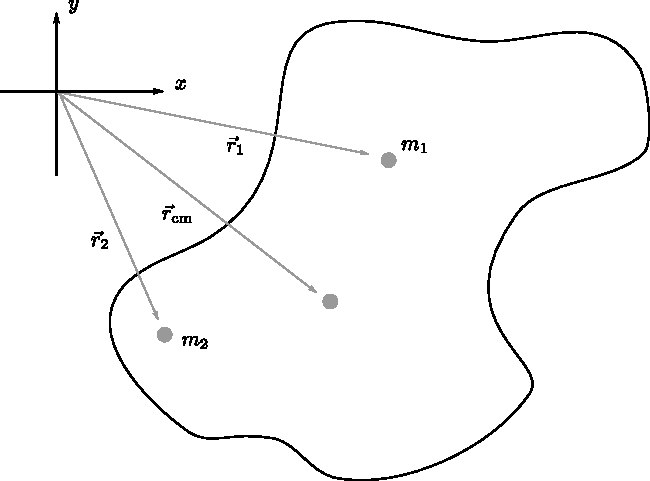
\includegraphics[scale = 1]{figures/cm1.pdf}
    \caption{Við getum skipt stjörfum hlut upp í punktmassa og fundið þannig massamiðju hlutarins.}
    \label{fig:cm1}
\end{figure}

Þetta væri mjög gagnlegt ef að hlutirnir okkar væru allir punktmassar. Hinsvegar, ef við ætlum að finna massamiðju hlutar sem er samanhangandi t.d.~eins og diskur, spýta eða bók þá vandast málin. Því þá þyrftum við að nota skilgreininguna hérna að ofan fyrir hvert einasta atóm í hlutnum! Til þess að auðvelda okkur slíka reikninga til að finna massamiðjur samfelldra hluta þá nota menn svokallaðan tegurreikning (sem þið lærið í 6. bekk í MR). En það er oft líka hægt að nota eðlisfræðileg innsæi (einnig þekkt sem \duck{common sense}) til þess að finna massamiðjur stífrahluta. Til dæmis vitum við að massamiðja einsleitrar kúlu er í miðjunni á kúlunni. Við vitum einnig að massamiðja einsleitrar stangar er í miðju stangarinnar. Ástæðan fyrir því að við höfum svona mikinn áhuga á massamiðjunni er vegna eftirfarandi tveggja lögmála:

\begin{tcolorbox}
\begin{theorem}
Lýsa má hreyfingu stjarfhlutar í heild sinni út frá hreyfingu massamiðjunnar.
\end{theorem}
\end{tcolorbox}

\textbf{Útleiðsla:} Þetta fæst með örlítilli umritun á skilgreiningunni á massamiðjunni:
\begin{align*}
    M\vec{r}_{\text{cm}} = \sum_{i=1}^{n} m_i \vec{r}_i \implies M \vec{v}_{\text{cm}} = \sum_{i=1}^{n} m_i \vec{v}_i \implies  M \vec{a}_{\text{cm}} = \sum_{i=1}^{n} m_i \vec{a}_i.
\end{align*}
En þetta þýðir að við höfum að heildarskriðþungi kerfisins er gefinn með:
\begin{align*}
    \vec{p}_{\text{heild}} = \sum_{i=1}^{n} m_i \vec{v}_i = M\vec{v}_{\text{cm}}.
\end{align*}
Eins sýnir þetta að heildarkrafturinn sem verkar á kerfið gefinn með:
\begin{align*}
    \vec{F}_{\text{heild}} = \frac{dp_{\text{heild}}}{dt} = \sum_{i=1}^{n} m_i \vec{a}_i = M\vec{a}_{\text{cm}}.
\end{align*}
\qed

Við sjáum einnig að ef heildarkrafturinn sem verkar á stjarfan hlut er núll þá er heildarskriðþungi stjarfhlutarins varðveittur. Annað sem við sjáum er að ef $U_i = m_igh_i$ táknar stöðuorku hvers punktmassa fyrir sig þá er heildarstöðuorkan gefin með:
\begin{align*}
    U_{\text{heild}} = \sum_{i=1}^{n} m_igh_i = g \sum_{i=1}^{n}m_i h_i = g Mh_{\text{cm}} = Mgh_{\text{cm}}.
\end{align*}

Við munum síðan síðar sýna að:

\begin{tcolorbox}
\begin{theorem}
Hlutir snúast um massamiðju sína nema þeir séu neyddir til þess að snúast öðruvísi.
\end{theorem}
\end{tcolorbox}

Við minnumst að lokum á eftirfarandi niðurstöðu sem sýnir okkur hvernig við getum fundið massamiðjur samsettra hluta (sem samanstanda af mörgum stífum hlutum).


\begin{tcolorbox}
\begin{theorem}
Látum $A$ vera stjarfan hlut með massamiðju $\vec{r}_A$ og heildarmassa $m_A$ og látum $B$ vera stjarfan hlut með massamiðju $\vec{r}_B$ og heildarmassa $m_B$. Massamiðja samsetta hlutarins $AB$ er þá:
\begin{align*}
    \vec{r}_{\text{cm}} = \frac{m_A \vec{r}_A+m_B\vec{r}_B}{m_A + m_B}.
\end{align*}
\end{theorem}
\end{tcolorbox}

\begin{figure}[H]
    \centering
    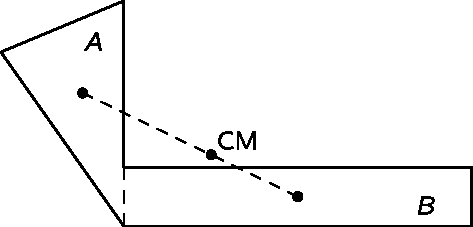
\includegraphics[scale=1]{figures/feyncm.pdf}
    \caption{Þegar við setjum saman tvo stjarfa hluti þá er auðvelt að finna massamiðjur þeirra.}
    \label{fig:feyncm}
\end{figure}


\section{Hverfitregður og snúningsásar}

\begin{tcolorbox}
\begin{definition}
Við segjum að vigur $\vec{s} \in R^3$ sé \textbf{snúningsás} fyrir kerfi ef kerfið snýst með jákvæðum snúning umhverfis snúningsásinn.
\end{definition}
\end{tcolorbox}

Það eru margar leiðir til að snúa hlut svo í rauninni geta allir vigrar $\vec{s} \in \R^3$ verið snúningsás fyrir hlutinn. Snúningsásinn getur legið í gegnum hlutinn en snúningsásinn getur einnig legið fyrir utan hlutinn. 

\begin{tcolorbox}
\begin{definition}
Lítum á punktmassa $m$ sem er í fjarlægð $r$ frá snúningsás $\vec{s}$. \textbf{Hverfitregða} punktmassans um snúningsásinn er táknuð með $I$ og skilgreind þannig að:
\begin{align*}
    I = mr^2.
\end{align*}
\end{definition}
\end{tcolorbox}

\begin{figure}[H]
    \centering
    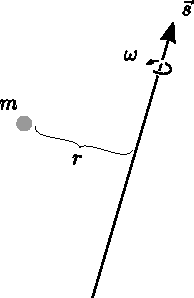
\includegraphics[scale=1.2]{figures/hverfi.pdf}
    \caption{Punktmassi $m$ í fjarlægð $r$ frá snúningsásnum, $\vec{s}$, hefur hverfitregðu $I = mr^2$.}
    \label{fig:hverfi}
\end{figure}
Við athugum að SI-einingar hverfitregðu eru gefnar með: $[I] = [mr^2] = \si{kgm^2}$. Við hugsum um hverfitregðuna sem mælikvarða á það hversu erfitt er að snúa massanum $m$ umhverfis snúningsásinn í fjarlægð $r$ frá honum. Sumir nota orðið snúningsmassi í staðinn fyrir orðið hverfitregða.

Það er hinsvegar erfitt að teikna þrívíða hluti á blaði svo við veljum oftast sjónarhorn í dæmunum okkar þannig að snúningsásinn liggji í stefnuna þvert á blaðið, annað hvort inn í blaðið eða út úr því. Því er þægilegt að taka upp myndrænan rithátt til að lýsa slíkum snúningsásum á myndum.

\begin{figure}[H]
    \centering
    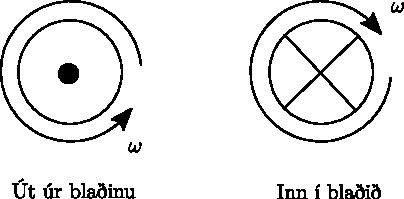
\includegraphics{figures/haegri.pdf}
    \caption{Í mörgum dæmum þá liggur snúningsásinn annað hvort inn í blaðið eða út úr því.}
    \label{fig:orvar}
\end{figure}

Ástæðan sem liggur að baki þessum rithætti sem við sjáum á mynd \ref{fig:orvar} er að við erum að hugsa um ör. Vinstri myndin sýnir þá örvaroddinn koma í áttina að okkur og hægri myndin sýnir síðan stélið á örinni fjarlægjast okkur.

\newpage

En stjarfir hlutir eru ekki punktmassar. En við getum 
Við höfum hinsvegar áhuga á því að finna hverfitregður stjarfra hluta um tiltekna snúningsása.

\begin{tcolorbox}
\begin{definition}
Lítum á stjarfan hlut með heildarmassa $m$. Látum $\vec{s}$ vera snúningsás. Hugsum okkur að við smættum hlutinn upp í punktmassa. Segjum sem svo að hluturinn skiptist upp í $n$ punktmassa sem hver um sig hefur örlítinn massa $dm_i$ og er í fjarlægð $r_i$ frá snúningsásnum. Við segjum að hverfitregða stjarfa hlutarins um snúningsásinn sé summan af hverfitregðum punktmassanna sem hluturinn samanstendur af. Með öðrum orðum þá höfum við að:
\begin{align*}
    I = dm_1r_1^2 + dm_2r_2^2 + \ldots + dm_n r_n^2 = \sum_{i=1}^{n} r_i^2 dm_i = \int r^2dm.
\end{align*}
\end{definition}
\end{tcolorbox}

Hér höfum við í síðasta skrefinu innleitt shorthand-ritháttinn $\int r^2dm$ í staðinn fyrir summuna $\sum\limits_{i=1}^{n}r_i^2dm_i$. Þetta er til að spara blýið í skriffærunum okkar (og pennanum mínum) og ekki eitthvað til þess að óttast.


\begin{tcolorbox}
\begin{theorem}
\textbf{(Regla Steiners)} Lítum á stjarfan hlut með heildarmassa $m$. Látum $\vec{s}_1$ og $\vec{s}_2$ vera samsíða snúningsása þannig að $\vec{s}_1$ liggur í gegnum massamiðju stjarfa hlutarins. Látum vegalengdina milli snúningsásanna vera $d$ og látum hverfitregðuna um snúningsásinn $\vec{s}_1$ vera $I_{\text{cm}}$ og hverfitregðuna um snúningsásinn $\vec{s}_2$ vera $I$. Þá gildir að:
\begin{align*}
    I = I_{\text{cm}} + md^2
\end{align*}
\end{theorem}
\end{tcolorbox}

\begin{figure}[H]
    \centering
    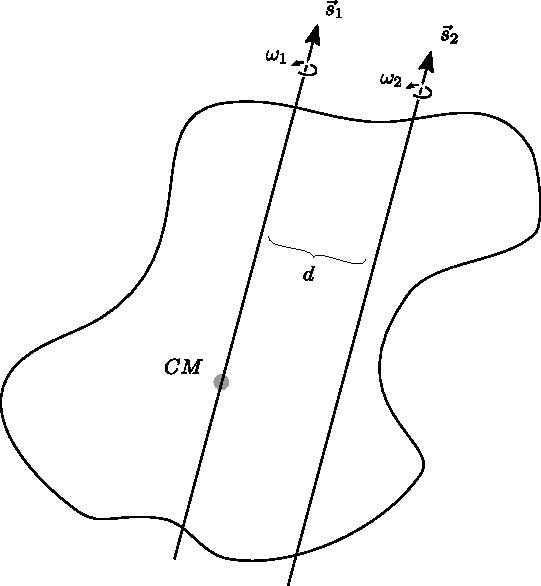
\includegraphics[scale=1]{figures/steiner2.pdf}
    \caption{Snúningsásarnir $\vec{s}_1$ og $\vec{s}_2$ eru samsíða og $\vec{s}_1$ liggur í gegnum massamiðju stjarfa hlutarins.}
    \label{fig:steiner}
\end{figure}

\newpage

\section{Hverfitregður algengra hluta}

\begin{table}[h!]
  \centering
  \begin{tabular}{ | c | m{5cm} | m{5cm} | }
    \hline
    Mynd & Lýsing & Hverfitregða \\ \hline
    \begin{minipage}{.3\textwidth}
    \vspace{0.3cm}
    \centering
      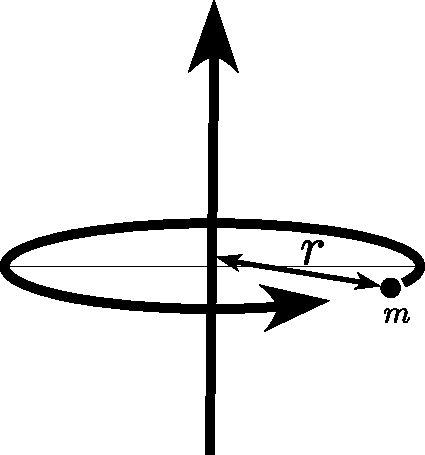
\includegraphics[width=0.7\linewidth]{momentsOfInertia/PointInertia.pdf}
    \vspace{0.3cm}
    \end{minipage}
    &
      Punktmassi með massa $m$ í fjarlægð $r$ frá snúningsásnum.
    & 
      \begin{align*}
          I = mr^2
      \end{align*}
    \\ \hline
        \begin{minipage}{.3\textwidth}
        \vspace{0.3cm}
    \centering
      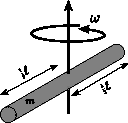
\includegraphics[width=0.8\linewidth]{momentsOfInertia/Moment_of_inertia_rod_center.pdf}
      \vspace{0.3cm}
    \end{minipage}
    &
      Einsleit stöng af lengd $\ell$ með massa $m$ um snúningsás sem liggur þvert í gegnum miðju stangarinnar.
    & 
      \begin{align*}
          I_{\text{cm}} = \frac{1}{12}m\ell^2
      \end{align*}
    \\ \hline
            \begin{minipage}{.27\textwidth}
        \vspace{0.3cm}
    \centering
      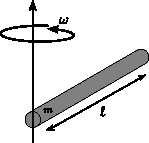
\includegraphics[width=0.75\linewidth]{momentsOfInertia/Moment_of_inertia_rod_end.pdf}
      \vspace{0.3cm}
    \end{minipage}
    &
      Einsleit stöng af lengd $\ell$ með massa $m$ um snúningsás sem liggur þvert í gegnum annan enda stangarinnar.
    & 
      \begin{align*}
          I_{\text{endi}} = \frac{1}{3}m\ell^2
      \end{align*}
    \\ \hline
                        \begin{minipage}{.3\textwidth}
        \vspace{0.3cm}
    \centering
      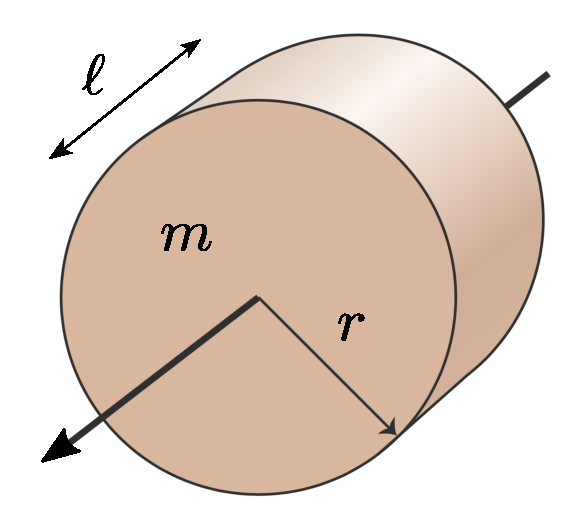
\includegraphics[width=0.75\linewidth]{momentsOfInertia/gsivaln.pdf}
      \vspace{0.3cm}
    \end{minipage}
    &
      Gegnheil sívalningur með geisla $r$, lengd $\ell$ og massa $m$ um snúningsás sem liggur í gegnum miðju sívalningsins.
    & 
      \begin{align*}
          I_{\text{cm}} = \frac{1}{2}mr^2
      \end{align*}
    \\ \hline
                \begin{minipage}{.3\textwidth}
        \vspace{0.3cm}
    \centering
      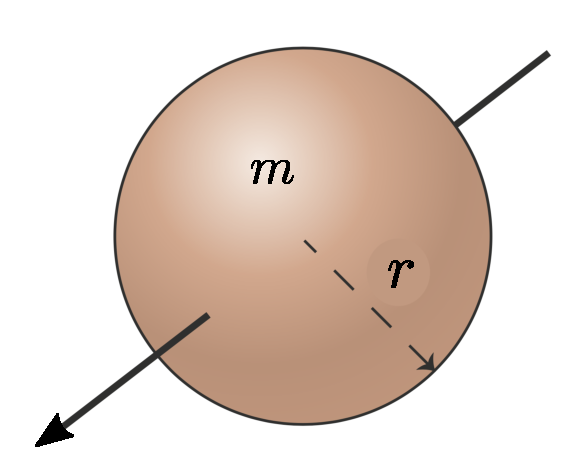
\includegraphics[width=0.75\linewidth]{momentsOfInertia/gkula.pdf}
      \vspace{0.3cm}
    \end{minipage}
    &
      Gegnheil kúla með geisla $r$ og massa $m$ um snúningsás sem liggur í gegnum miðju kúlunnar.
    & 
      \begin{align*}
          I_{\text{cm}} = \frac{2}{5}mr^2
      \end{align*}
    \\ \hline
    
    
  \end{tabular}
  \caption{Hverfitregður nokkurra algengra hluta} \label{table:hverfi}
\end{table}


\section{Útleiðslur á nokkrum hverfitregðum}

Fyrir stöngina þá er þægilegt að byrja á því að reikna hverfitregðuna um annan enda stangarinnar. Við athugum að stöngin hefur línulegan eðlismassa $\rho = \frac{m}{\ell}$. Hugsum okkur nú að við skiptum stönginni niður í litla búta þar sem hver bútur hefur þykkt $dx$. Þá er massinn í hverjum bút gefinn með $dm = \rho dx$ og við fáum samkvæmt skilgreiningu að:
\begin{align*}
    I = \int x^2dm = \int_{0}^{\ell}  x^2 \rho dx =  \left[ \frac{\rho}{3}x^3 \right]_{0}^{\ell} = \frac{\rho}{3}\left( \ell^3 - 0^3 \right) = \frac{\rho}{3}\ell^3 = \frac{1}{3}m\ell^2
\end{align*}
Þar sem við notuðum í síðasta skrefinu að $\rho = \frac{m}{\ell}$.

\begin{figure}[H]
    \centering
    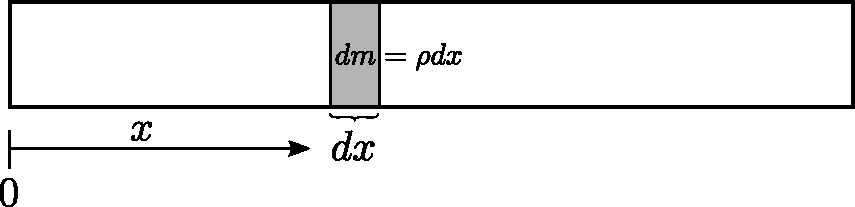
\includegraphics[scale=0.5]{momentsOfInertia/stongendi.pdf}
    \caption{Stönginni er skipt í litla punktmassa með massa $dm = \rho dx$ í fjarlægð $x$ frá enda stangarinnar.}
\end{figure}
Við getum síðan notað Reglu Steiners til að finna hverfitregðuna um massamiðju stangarinnar (hér erum við að nota að snúningsásarnir eru samsíða!). En þá höfum við að:
\begin{align*}
    I_{\text{enda}} = I_{\text{cm}} + md^2
\end{align*}
En í okkar tilviki er $d = \frac{\ell}{2}$ svo við fáum að:
\begin{align*}
    I_{\text{cm}} = I - md^2  = I_{\text{enda}} - m\left( \frac{\ell}{2} \right)^2 = \frac{1}{3}m\ell^2 - \frac{1}{4}m\ell^2 = \frac{1}{12}m\ell^2.
\end{align*}
Það er ágætt að minna sig á að lögmál Steiners segir okkur að hverfitregðan er alltaf lægst um massamiðjuna. Í okkar tilviki sjáum við að $\frac{1}{12} < \frac{1}{3}$ eins og við var að búast. \\

Við skulum núna finna hverfitregðu sívalningsins um ás sem liggur í gegnum massamiðjuna. Við skiptum gegnheila sívalningnum upp í litlar gjarðir af þekkt $dr$ og í fjarlægð $r$ frá miðju sívalningsins. Við athugum að eðlismassi sívalningsins á flatareiningu er þá gefinn með $\rho = \frac{m}{\pi R^2}$. Hver gjörð hefur þá massa $dm = 2\pi \rho r dr$ og við fáum að:
\begin{align*}
    I = \int r^2 dm = \int_{0}^{R} 2\pi \rho r^3 dr = \left[ \frac{1}{2}\pi \rho r^4  \right]_{0}^{R} = \frac{\pi \rho}{2}\left(R^4 - 0^4 \right) = \frac{1}{2}mR^2
\end{align*}

\begin{figure}[H]
    \centering
    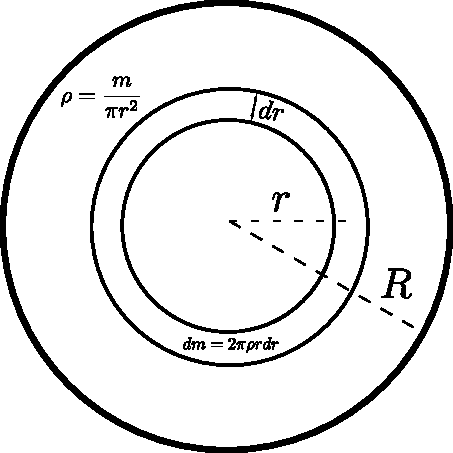
\includegraphics[scale=0.6]{momentsOfInertia/sivalninertia.pdf}
    \caption{Sívalningnum er skipt upp í þunnar gjarðir með þykkt $dr$ í fjarlægð $r$ frá miðju sívalningsins.}
\end{figure}


\begin{comment}
Að lokum skulum við reikna hverfitregðu kúlunnar. Við athugum að hún hefur eðlismassa $\rho = \frac{m}{\frac{4}{3}\pi R^3}$. Nú skiptum við kúlunni upp í kúluskeljar af þykkt $dr$. Við höfum þá að massinn í hverri kúluskel er gefinn með $dm = \rho 4\pi r^2 dr$ og við fáum að:
\begin{align*}
    I = \int r^2 dm = \int_{0}^{R} 4\pi \rho r^4 dr = \left[ \frac{4\pi \rho}{5} r^5 \right]_{0}^{R} = \frac{4\pi \rho}{5} \left( R^5 - 0^5 \right) = \frac{4\pi}{5} \frac{m}{\frac{4}{3}\pi R^3} R^5 = \frac{3}{5} mR^2.
\end{align*}
\end{comment}

\newpage

\section{Kraftvægi}

\begin{tcolorbox}
\begin{definition}
Lítum á tvo vigra $\Vec{a} = \smqty(a_x \\ a_y \\ a_z)$ og $\Vec{b} = \smqty(b_x \\ b_y \\ b_z)$. \textbf{Krossfeldi} vigranna $\Vec{a}$ og $\Vec{b}$ er táknað með $\Vec{a} \times \Vec{b}$, og skilgreint þannig að:
\begin{align*}
    \Vec{a} \times \Vec{b} = \begin{pmatrix}
    a_y b_z - a_z b_y \\
    a_zb_x - a_x b_z \\
    a_x b_y - a_y b_x
    \end{pmatrix}
\end{align*}
\end{definition}
\end{tcolorbox}

\begin{figure}[H]
    \centering
    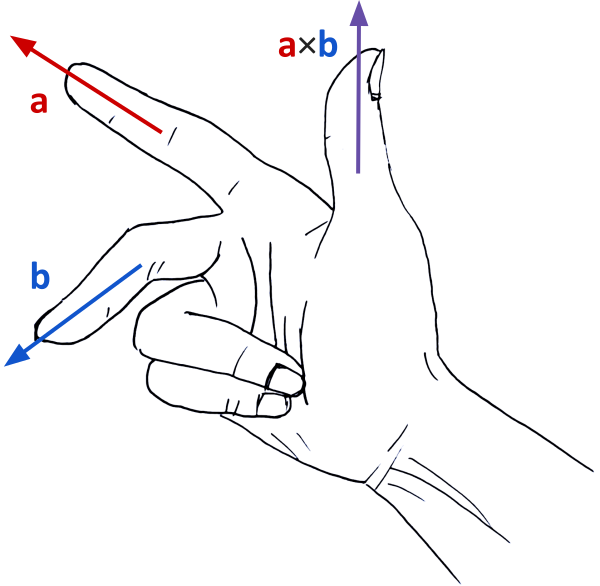
\includegraphics[scale = 0.2]{temp/hhr.png}
    \caption{Við getum ákvarðað stefnu krossfeldisins með svokallaðri hægri handar reglu.}
    \label{fig:rhr}
\end{figure}

En eins og með innfeldi vigra þá er til þægilegri leið til þess að hugsa um krossfeldið. Við höfum nefnilega:

\begin{tcolorbox}
\begin{setning}
Látum $\Vec{a}, \Vec{b} \in \R^3$. Látum hornið milli vigranna $\Vec{a}$ og $\Vec{b}$ vera $\varphi$. Þá gildir að:
\begin{align*}
    \abs{\Vec{a} \times \Vec{b}} = ab\sin\varphi.
\end{align*}
Þar sem að $a = \abs{\Vec{a}}$ og $b = \abs{\Vec{b}}$.
\end{setning}
\end{tcolorbox}

\textbf{Sönnun:} Við getum valið hnitakerfið þannig að vigrarnir $\Vec{a}$ og $\Vec{b}$ liggi í $xy$-planinu. Þá er $\Vec{a} = \smqty(a_x \\ a_y \\ 0)$ og eins er $\Vec{b} = \smqty(b_x \\ b_y \\ 0)$. Þá sjáum við að krossfeldi vigranna verður $\Vec{a} \times \Vec{b} = \smqty(0 \\ 0 \\ a_x b_y - a_y b_x)$. Skrifum síðan $\Vec{a} = \smqty(a\cos\alpha \\ a\sin\alpha \\ 0)$ og $\Vec{b} = \smqty(b\cos\beta \\ b\sin\beta \\ 0)$, þar sem $\alpha$ og $\beta$ eru stefnuhorn vigranna $\vec{a}$ og $\vec{b}$. Þá höfum við að:
\begin{align*}
    \abs{\Vec{a}\times \Vec{b}}^2 = \left(a_xb_y - a_y b_x\right)^2  = a^2b^2 \left( \cos\alpha \sin\beta - \sin\alpha \cos\beta \right)^2 = a^2b^2 \sin^2(\alpha - \beta) = a^2b^2\sin^2\gamma
\end{align*}
Þar sem að $\gamma = \alpha - \beta$ er hornið milli vigranna $\Vec{a}$ og $\Vec{b}$. Þar með höfum við sýnt að $\abs{\Vec{a}\times \Vec{b}} = ab\sin\gamma$. \qed


\begin{tcolorbox}
\begin{definition}
Lítum á stjarfan hlut sem verður fyrir krafti $\vec{F}$ í fjarlægð $\vec{r}$ frá snúningsás hlutarins. \textbf{Kraftvægi} kraftsins $\vec{F}$ er táknað með $\vec{\tau}$ og skilgreint þannig að:
\begin{align*}
    \vec{\tau} = \vec{r} \times \vec{F}.
\end{align*}
\end{definition}
\end{tcolorbox}

Röðin skiptir máli! Við athugum að þá er stærðin á kraftvæginu gefin með $\tau = rF\sin\varphi$, þar sem $\varphi$ er hornið milli $\vec{r}$ og $\vec{F}$. Við höfum síðan að $2.$ lögmál Newtons fyrir snúninga verður:

\begin{tcolorbox}
\begin{theorem}
\textbf{(2. lögmál Newtons fyrir snúninga)} 
\begin{align*}
    \tau_{\text{heild}} = \tau_1 + \tau_2 + \ldots + \tau_n = I \alpha.
\end{align*}
\end{theorem}
\end{tcolorbox}


\section{Hverfiþungi}

Hliðstæða skriðþungans $p = mv$ er hverfiþunginn.
\begin{tcolorbox}
\begin{definition}
Lítum á stjarfan hlut sem hefur hverfitregðu $I$ og hornhraða $\omega$ um tiltekinn snúningsás. \textbf{Hverfiþungi} hlutarins um snúningsásinn er þá skilgreindur þannig að
\begin{align*}
    L = I\omega.
\end{align*}
\end{definition}
\end{tcolorbox}

Það er reyndar önnur leið til þess að skilgreina hverfiþunga, en hún gildir fyrir hvern stakan punktmassa. Við höfum nefnilega að:

\begin{align*}
    \vec{L} = \vec{r}\times \vec{p}
\end{align*}
Fyrir punktmassa. Við sjáum að ef $\vec{p}$ og $\vec{r}$ eru hornréttir þá fæst einmitt að $L = rmv = mvr$. En fyrir punktmassa höfum við einmitt líka að $L = I\omega = mr^2 \frac{v}{r} = mvr$. Við sjáum líka að ef við skiptum hlut niður í litla búta þá höfum við að:
\begin{align*}
    \vec{L} = \sum_{i=1}^{n} \vec{r}_i \times \vec{p}_i =  \sum_{i=1}^{n} \vec{r}_i \times \vec{p}_i = \sum_{i=1}^{n} m_i \vec{r}_i \times \vec{v}_i = \sum_{i=1}^{n} m_i r_i v_i \frac{\vec{\omega}}{\omega} = \vec{\omega} \sum_{i=1}^{n}m_i r_i^2 = I\vec{\omega}.
\end{align*}



\begin{tcolorbox}
\begin{theorem}
\textbf{(Hverfiþungavarðveisla)} Heildarhverfiþungi kerfis er varðveittur ef engin ytri kraftvægi verka á kerfið. Með öðrum orðum, ef $L_{\text{fyrir}}$ táknar hverfiþunga kerfis við tíma $t_1$ og $L_{\text{eftir}}$ táknar hverfiþunga kerfis eftir tíma $t_2$. Þá gildir að:
\begin{align*}
    L_{\text{fyrir}} = L_{\text{eftir}}.
\end{align*}
\end{theorem}
\end{tcolorbox}

\textbf{Útleiðsla:} Við athugum að:
\begin{align*}
    \frac{d\vec{L}}{dt} = \frac{d}{dt}\left( \vec{r} \times \vec{p} \right) = \explain{\dot{\vec{r}} \times \vec{p}}{=0} + \vec{r}\times \dot{\vec{p}} = \vec{r}\times \vec{F} = \vec{\tau}.
\end{align*}
Við ályktum því að ef $\vec{\tau} = 0$ þá er $\frac{d\vec{L}}{dt} = 0$, þ.e.a.s.~að hverfiþunginn varðveittur. \qed

\section{Snúningsorka}

\begin{tcolorbox}
\begin{definition}
Lítum á hlut með geisla $r$ sem snýst um massamiðju sína með hornhraða $\omega$. Við segjum að hluturinn \textbf{rúlli án þess að renna} ef við höfum að:
\begin{align*}
    v_{\text{cm}} = r\omega, \hspace{0.8cm} \text{og} \hspace{0.8cm} a_{\text{cm}} = r\alpha.
\end{align*}
\end{definition}
\end{tcolorbox}
Það er algengt að fólk misskilji þetta þar sem að þetta lítur eins út og jafna sem við höfðum leitt út áður, nefnilega að $v = r\omega$. En sú niðurstaða gildir fyrir punkta á jaðri hringsins í fjarlægð $r$ frá miðju hringsins. Þessi niðurstaða gildir hinsvegar fyrir hraðann á massamiðju hlutarins, $v_{\text{cm}}$. Það er hægt að leiða þetta út með því að skoða vegalengdina sem að massamiðjan ferðast á þeim tíma þar sem að hluturinn er að snúast einn hring. Þá höfum við að vegalengdin sem að punktur á gjörðinni ferðast er $s = 2\pi r$ og tíminn sem það tekur er $T = \frac{2\pi}{\omega}$. Ef hluturinn rúllar án þess að renna þá er vegalengdin sem massamiðjan ferðast á þeim tíma einnig gefin með $s_{\text{cm}} = 2\pi r$ svo við fáum að
\begin{align*}
    v_{\text{cm}} = \frac{s_{\text{cm}}}{T} = \frac{2\pi r}{\frac{2\pi}{\omega}} = r \omega.
\end{align*}


Þegar hlutir snúast hafa þeir bæði hreyfiroku vegna þess hversu hratt hluturinn er að ferðast og hreyfiorku vegna þess hve hratt hluturinn er að snúast þessu má lýsa þannig að hreyfiorka hlutarins er gefin með:

\begin{tcolorbox}
\begin{definition}
Lítum á stjarfan hlut með massa $m$ og hverfitregðu $I$. Látum massamiðju hlutarins hafa línulegan hraða $v_{\text{cm}}$ og látum hlutinn snúast um snúningsás sem liggur í gegnum massamiðjuna með hornhraða $\omega$. Þá er hreyfiorka hlutarins gefin með:
\begin{align*}
    K = K_{\text{hreyfi}} + K_{\text{snúnings}} = \frac{1}{2}mv_{\text{cm}}^2 + \frac{1}{2}I_{\text{cm}}\omega^2
\end{align*}
\end{definition}
\end{tcolorbox}

Að lokum skulum við athuga að:

\begin{comment}
Í því sértilfelli að hlutur rúllar án þess að renna þá höfum við að $v_{\text{cm}} = r \omega $ og því $\omega = \frac{v_{\textrm{cm}}}{r}$ og ef að við skrifum $I = \sigma mr^2$ þá fáum við að:
\begin{align*}
    K = \frac{1}{2}mv_{\text{cm}}^2 + \frac{1}{2}I_{\text{cm}}\omega^2 = \frac{1}{2}mv_{\text{cm}}^2 + \frac{1}{2}\sigma mr^2 \left( \frac{v_{\text{cm}}}{r}\right)^2 = \frac{1}{2} \left(1 + \sigma\right) mv_{\text{cm}}^2.
\end{align*}
\end{comment}

\begin{tcolorbox}
\begin{theorem}
Lítum á stjarfan hlut sem verður fyrir föstu kraftvægi $\vec{\tau}$ í fjarlægð $\vec{r}$ frá miðju snúningsássins vegna fasta kraftsins $\vec{F}$. Þá er vinna kraftvægisins, $\tau$, við það að flytja hlutinn um horn $\Delta \theta$ gefin með:
\begin{align*}
    W = \tau \Delta \theta.
\end{align*}
\end{theorem}
\end{tcolorbox}

\textbf{Útleiðsla:} Við vitum að $W = \Delta K$. Eina breytingin sem verður í hreyfiorkunni er í snúningsorkuliðnum. Við höfum því að:
\begin{align*}
    W = \Delta K = \frac{1}{2}I \omega^2 - \frac{1}{2}I\omega_0^2 = \frac{1}{2}I\left( \omega^2 - \omega_0^2 \right)
\end{align*}
En þar sem að vægið er fast þá höfum við að hornhröðun hlutarins, $\alpha$, er föst. En þar með gilda hornstöðujöfnurnar okkar svo við höfum að:
\begin{align*}
    \omega = \omega_0 + \alpha t
\end{align*}
Við stingum því inn í vinnuna og fáum að:
\begin{align*}
    W = \frac{1}{2}I\left( (\omega_0 + \alpha t)^2 - \omega_0^2 \right) = \frac{1}{2}I \left( 2\omega_0 \alpha t + \alpha^2 t^2 \right) = I\alpha \left( \omega_0 t + \frac{1}{2}\alpha t^2 \right) = I\alpha \Delta \theta = \tau \Delta \theta.
\end{align*}
\qed


\section*{Samantekt}

\begin{table}[H]
\begin{center}
\begin{tabular}{|c|c|}
\hline
\textbf{Línuleg hreyfing} & \textbf{Snúningshreyfing} \\
\hline
$v = \frac{ds}{dt} $ & $\omega = \frac{d\theta}{dt}$ \\
$a = \frac{dv}{dt} $ & $\alpha = \frac{d\omega}{dt}$ \\
$s = s_0 + v_0t + \frac{1}{2}at^2 $ & $\theta = \theta_0 + \omega_0 t + \frac{1}{2}\alpha t^2$ \\
$v = v_0 + a t$ & $\omega = \omega_0 + \alpha t$ \\
$2a \Delta s = v^2 - v_0^2$ & $2 \alpha \Delta \theta = \omega^2 - \omega_0^2$  \\
\hline
\end{tabular}
\caption{Stöðujöfnurnar fyrir snúning og línulega hreyfingu.}
\label{tafla:raddi}
\end{center}
\end{table}

\begin{table}[H]
\begin{center}
\begin{tabular}{|c|c|}
\hline
\textbf{Línuleg hreyfing} & \textbf{Snúningshreyfing} \\
\hline
$F = ma = \frac{dp}{dt} $ & $\tau = I\alpha = rF\sin\varphi = \frac{dL}{dt}$ \\
$F_{\text{heild}} = F_1 + \ldots + F_n $ & $\tau_{\text{heild}} = \tau_1 + \ldots + \tau_n$ \\
$p = mv $ & $L = I\omega = rp\sin\varphi$ \\
$K = \frac{1}{2}mv^2$ & $K_{\text{snú}} = \frac{1}{2}I\omega^2$ \\
$W = Fd\cos\gamma$ & $W = \tau \Delta \theta$ \\
\hline
\end{tabular}
\caption{Hliðstæðar jöfnur fyrir línulega hreyfingu og snúningshreyfingu.}
\label{tafla:laddi}
\end{center}
\end{table}



\section{Sýnidæmi}

\subsection*{Trissa sem er ekki massalaus}

Skoðum núna aftur uppstillinguna í tilrauninni togkraftur og hröðun.

\begin{figure}[H]
    \centering
    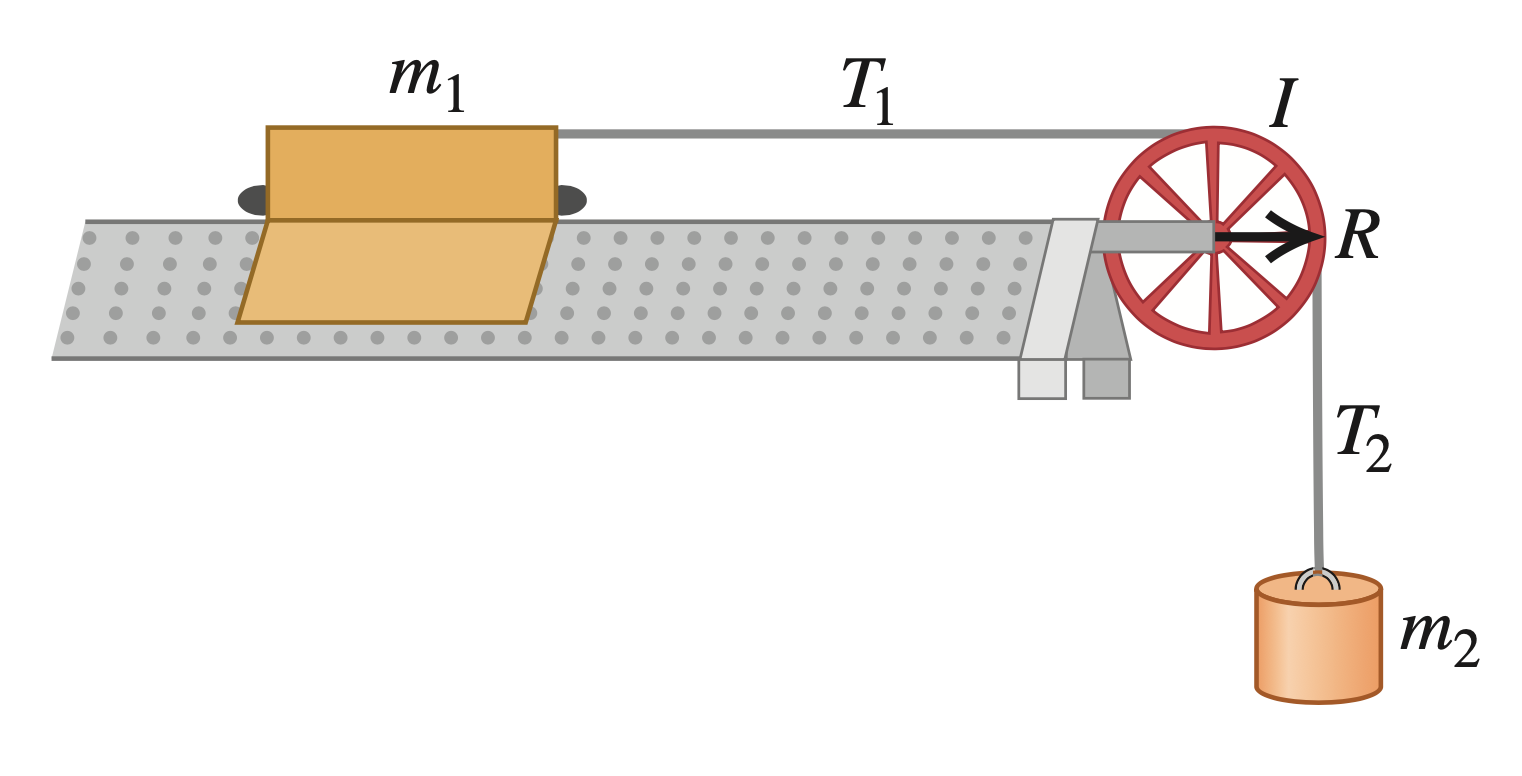
\includegraphics[width=0.65\textwidth]{images/togkrafturoghverfitregda.png}
\end{figure}

Við skrifum niður kraftajöfnurnar fyrir massana:

\begin{align*}
    \begin{pmatrix} m_1 a \\ 0 \end{pmatrix} = \begin{pmatrix}  T_1 - F_{\text{nún}} \\ Þ - m_1g \end{pmatrix}
\end{align*}
Síðan höfum við:
\begin{align*}
   m_2 a = m_2g - T_2
\end{align*}
Þegar trissan er massalaus þá getum við sagt að $T_1 = T_2$. En núna verður þetta flóknara og við munum fá að $T_1 \neq T_2$ þar sem að trissan hefur massa. Við höfum eftirfarandi vægisjöfnu fyrir trissuna:
\begin{align*}
    \tau_{\text{heild}} = I\alpha = T_2 R - T_1 R = (T_2-T_1)R
\end{align*}
Við notum síðan að $\alpha = \frac{a}{R}$ og þá höfum við eftirfarandi jöfnuhneppi:
\begin{align*}
    \begin{cases}
    m_1a = T_1 - \mu m_1 g \\
    m_2a = m_2g - T_2 \\
    Ia = (T_2 - T_1)R^2
    \end{cases}
\end{align*}
Við notum þá sama samlagningartrikk og áður. Við leggjum saman efri tvær jöfnurnar og fáum að:
\begin{align*}
    \left(m_1 + m_2\right)a = (T_1 - T_2) + \left( m_2 - \mu m_1\right)g
\end{align*}
Við færum síðan $(T_1 - T_2)$ yfir jafnaðarmerkið og umritum aðeins vægisjöfnuna þannig að $\frac{I}{R^2}a = T_2 - T_1$ og þá sjáum við að:
\begin{align*}
    \left(m_1 + m_2 + \frac{I}{R^2}\right)a = \left(m_2 - \mu m_1 \right)g \implies a = \left(\frac{m_2 - \mu m_1}{m_1 + m_2 + \frac{I}{R^2}} \right)g
\end{align*}
Við sjáum að þegar að trissan er massalaus, þ.e.a.s.~þegar $I = 0$ þá fáum við úr vægisjöfnunni að $T_2 = T_1$ eins og við notuðum óspart fyrir jól. Við sjáum einnig að þegar $I = 0$ þá fáum við gömlu hröðunina $a = \left(\frac{m_2 - \mu m_1}{m_1 + m_2}\right)g$ eins og við leiddum út fyrir jól fyrir massalausa trissu. Núna bætist hinsvegar við liður í nefnaranum. Það eina sem við eigum eftir á þessum tímapunkti er að finna hverfitregðu trissunnar (reyndar væri hægt að framkvæma tilraun til þess að ákvarða hverfitregðu trissunnar með uppsetningunni sem við notuðum í tilrauninni togkraftur og hröðun). Við vitum reyndar að hverfitregðan mun vera á forminu $I_{\text{trissa}} = \sigma mR^2$ þar sem $\sigma$ er snúningsstuðull trissunnar. Það þýðir að við getum einfaldað jöfnuna enn frekar þannig að:
\begin{align*}
    a = \left(\frac{m_2 - \mu m_1}{m_1 + m_2 + \sigma m}\right) g
\end{align*}
Þar sem að $m$ er massi trissunnar og $\sigma$ er snúningsstuðull hennar. Þessi trissa er reyndar undarleg í laginu (venjulega eru trissur bara sívalingslaga og með hverfitregðu $I = \frac{1}{2}mr^2$, þ.e.a.s.~með snúningsstuðull $\sigma = \frac{1}{2}$). Við þurfum aðeins að hafa fyrir því að finna hverfitregðuna 
á þessari trissu. Hún hefur heildarmassann $m$ og geislann $R$. Við sjáum við að hún er samsett úr þrem stöngum sem við snúum um miðju og gjörð sem er snúið um miðju. Ef allir hlutarnir eru jafnþykkir þá sjáum við að stangirnar hafa lengd $2R$ og gjörðin hefur ummál $2\pi R$ svo að línulegi eðlismassinn er gefinn með:
\begin{align*}
    \rho = \frac{m}{3\cdot 2R + 2\pi R} = \frac{m}{2R(3 + \pi)}
\end{align*}
En þá er heildarvægið gefið með:
\begin{align*}
    I =3 I_{\text{stöng}} + I_{\text{gjörð}} = 3 \cdot \frac{1}{12}(\rho 2R) R^2 + (\rho 2\pi R)R^2 = \left( \frac{1}{4(3+\pi)} + \frac{\pi}{(3+\pi)}  \right)mR^2 = \frac{1+4\pi}{4(3+\pi)} mR^2
\end{align*}
Við sjáum að $\sigma = \frac{1+4\pi}{4(3+\pi)} \approx 0.55$ í þessu tilviki.


\subsection*{Vél Atwoods þar sem trissan er hvorki massalaus né núningslaus}

Lítum núna aftur á vél Atwoods þar sem að 

\begin{figure}[H]
    \centering
    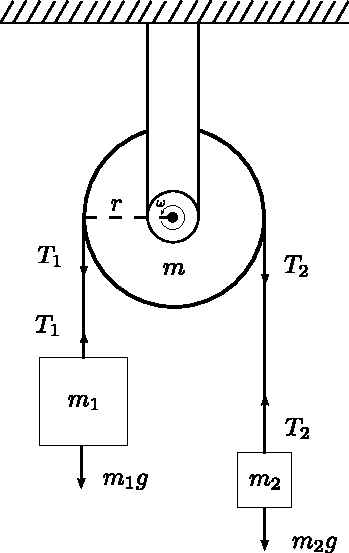
\includegraphics[scale=0.8]{figures/atwoodrot4.pdf}
\end{figure}

\begin{align*}
    m_1 a = m_1g - T_1
\end{align*}

\begin{align*}
    m_2a = T_2 - m_2g
\end{align*}
Loks höfum við vægisjöfnuna fyrir trissuna:
\begin{align*}
    I\alpha = (T_1 - T_2)r
\end{align*}
Við notum trikkið okkar og leggjum saman allar jöfnurnar (og notum að $\alpha = \frac{a}{r}$) til að fá:
\begin{align*}
    \left(m_1 + m_2 + \frac{I}{r^2}\right)a = \left(m_1 - m_2 \right)g
\end{align*}
Notum síðan að $I = \frac{1}{2}mr^2$ er hverfitregða trissunnar og fáum að:
\begin{align*}
    a = \frac{m_1 - m_2}{m_1 + m_2 + \frac{1}{2}m}g.
\end{align*}



\subsection*{Keilukúla sem rennur áður en hún byrjar að rúlla án þess að renna}

Ef þið hafið farið í keilu. Þá hafiði kannski tekið eftir því að keilukúlan byrjar fyrst á því að renna meðfram gólfinu þar til að rétt áður en að hún reikst á kúlukúlurnar þá byrjar hún að rúlla án þess að renna. Við ætlum að reyna að skýra þetta fyrirbæri hér. Hugsum okkur því keilukúlu með massa $m$ og geisla $r$ sem við köstum af stað þannig að massamiðja kúlunnar hefur línulegan hraða $v_0$ til að byrja með og hornhraði kúlunnar er $\omega_0 = 0$ í upphafi þegar kúlan leggur af stað niður keilubrautina. Við viljum ákvarða tímann $\tau$ sem líður þar til að kúlan byrjar að rúlla án þess að renna og vegalengdina $x$ sem kúlan hefur ferðast þá. 

\begin{figure}[H]
    \centering
    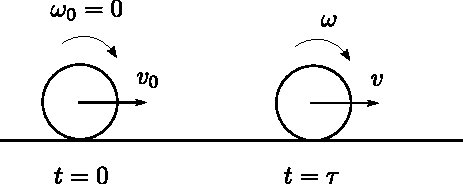
\includegraphics{figures/rullaogrenna.pdf}
\end{figure}

Það sem mun valda snúninginum er kraftvægið frá núningskraftinum. Núna er kúlan að renna meðfram yfirborðinu svo að kúlan finnur fyrir hreyfinúningi $F_{\text{nún}} = \mu Þ = \mu mg$ og hann veldur vægi á kúluna sem er gefið með:
\begin{align*}
    I\alpha = F_{\text{nún}}r
\end{align*}
En $I = \sigma mr^2$ þar sem $\sigma = \frac{2}{5}$ svo við höfum að:
\begin{align*}
    \sigma mr^2\alpha = \mu mgr \implies \alpha = \frac{\mu}{\sigma} \frac{g}{r}.
\end{align*}
Við höfum líka kraftajöfnuna fyrir keilukúluna:
\begin{align*}
    \begin{pmatrix} ma \\ 0 \end{pmatrix} = \begin{pmatrix} -F_{\text{nún}} \\ Þ - mg \end{pmatrix}
\end{align*}
Svo að hröðunin er gefin með $a = -\mu g$ svo að það hægist á kúlunni. Takið sérstaklega eftir því að það er ekki satt að $a = \alpha r = \frac{\mu}{\sigma}g$ því það gildir einungis þegar kúlan rúllar án þess að renna (þar erum við að nota að $v_{\text{cm}} = r\omega \implies a_{\text{cm}} = r\alpha$). Við sjáum að bæði hornhraði kúlunnar og hornhröðun hennar eru fastar stærðir svo að við vitum að við getum notað stöðujöfnurnar. Kúlan mun byrja að rúlla án þess að renna þegar $v_{\text{cm}} = r\omega$. Við notum því stöðujöfnurnar:
\begin{align*}
    \omega = \omega_0 + \alpha t, \hspace{1cm} v_{\text{cm}} = v_0 + a_{\text{cm}}t
\end{align*}
Þegar við setjum þetta saman þá fáum við að:
\begin{align*}
    v_{\text{cm}} = r\omega \implies v_0 + a_{\text{cm}}t = r\left( \omega_0 +\alpha t \right) \implies t = \frac{v_0}{\alpha r - a_{\text{cm}}} = \frac{v_0}{\frac{\mu}{\sigma}g + \mu g} = \frac{\sigma}{1+\sigma}\frac{v_0}{\mu g}
\end{align*}
Við ályktum því að tíminn, $\tau$, sé gefinn með:
\begin{align*}
    \tau = \frac{\sigma}{1+\sigma}\frac{v_0}{\mu g}
\end{align*}
Heildarvegalengdin sem kúlan hefur þá ferðast á þeim tímapunkti er þá gefin með:
\begin{align*}
    x = x_0 + v_0 t + \frac{1}{2}at^2 = v_0 \tau - \frac{1}{2}\mu g \tau^2.
\end{align*}
Við getum metið tölulegt gildi á þessum stærðum fyrir dæmigerða keilubraut. Núningurinn er frekar lítill í slikri braut svo að $\mu = \SI{0.1}{}$ og segjum að við köstum kúlunni með upphafshraða $\SI{7.5}{m/s}$. Heildarlengd keilubrautar er um það bil $d = \SI{20}{m}$. Loks er $\sigma = \frac{2}{5}$ fyrir keilukúlu svo við fáum að:
\begin{align*}
    \tau = \SI{2.18}{s}, \hspace{0.75cm} \text{og} \hspace{0.75cm} x = \SI{14.0}{m}
\end{align*}
Eftir það mun kúlan rúlla án þess að renna þar til hún rekst á keilupinnana. 


\subsection*{Hver vinnur kapphlaupið?}

\begin{figure}[H]
    \centering
    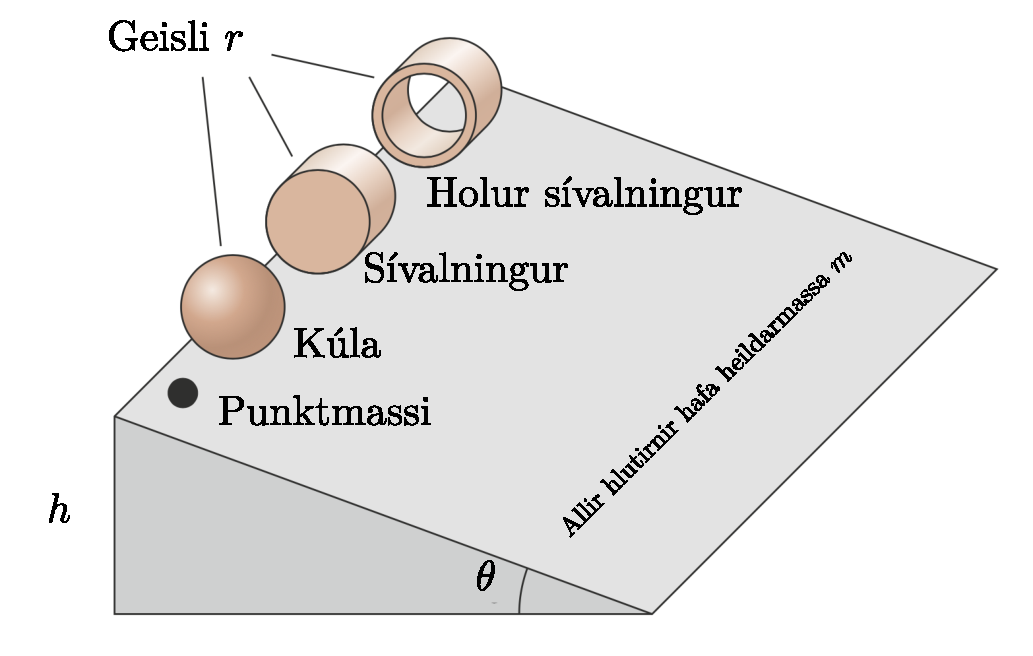
\includegraphics[scale=0.5]{figures/rullakeppni.pdf}
\end{figure}

Við höfum samkvæmt orkuvarðveislu að:
\begin{align*}
    mgh = K_{\text{hreyfi}} + K_{\text{snú}} = \frac{1}{2}mv_{\text{cm}}^2 + \frac{1}{2} I_{\text{cm}}\omega^2
\end{align*}
Við vitum að hlutirnir munu rúlla án þess að renna svo $v_{\text{cm}} = r\omega$ og ef við látum $I = \sigma mr^2$ þar sem $\sigma$ er snúningsstuðull hlutanna þá fáum við að:
\begin{align*}
    mgh = \frac{1}{2}mv_{\text{cm}}^2 + \frac{1}{2}\sigma mr^2 \left(\frac{v_{\text{cm}}}{r}\right)^2 = \frac{1}{2}\left(1+\sigma \right)mv_{\text{cm}}^2 
\end{align*}
En það gefur því að lokahraðinn þegar hlutirnir koma niður er gefinn með:
\begin{align*}
    v_{\text{cm}} = \sqrt{\frac{2gh}{(1+\sigma)}}
\end{align*}
Við sjáum því að því stærra sem $\sigma$ er því hægar kemur hluturinn í mark. Við höfum því að $\sigma_p = 0$ fyrri punktmassann svo hann sigrar. Síðan er $\sigma_k = \frac{2}{5}$ fyrir kúluna svo hún kemur næst í mark. Fyrir sívalninginn er $\sigma_s = \frac{1}{2}$ svo hann kemur næst í mark og loks er $\sigma_{hs} = 1$ fyrir hola sívalninginn svo hann kemur síðast í mark. Ástæðan sem liggur þarna að baki er að stöðuorkan breytist bæði í línulega hreyfiorku og í snúningsorku. Hversu mikið breytist í snúningsorku er háð snúningsstuðli hlutarins. Því meira sem breytist í snúningsorku því hægar kemur hluturinn í mark. Ef við erum ekki sátt með þessa skýringu þá getum við gefið aðra útskýringu sem við skulum sýna að er jafngild þessari sem við vorum að gefa. Við athugum þá að krafturinn sem veldur snúningnum í fyrsta lagi er núningskrafturinn. Við höfum þá kraftvægisjöfnuna:

\begin{align*}
   I\alpha = F_{\text{nún}}r
\end{align*}
og við notum síðan að $\alpha = \frac{a}{r}$ og að $I = \sigma mr^2$ til að fá að:
\begin{align*}
    F_{\text{nún}} = \sigma m a
\end{align*}
Það er reyndar algengur misskilningur sem á sér stað á þessu stigi málsins. Margir halda að $F_{\text{nún}} = \mu mg\cos\theta$ þar sem að $Þ = mg\cos\theta$. Það fyrra er ekki satt. Besta leiðin til að muna eftir því að þetta gildir ekki er að átta sig á því að hér erum við að glíma við kyrrstöðunúninginn en ekki hreyfinúninginn. Það er vegna þess að það er bara einn punktur á gjörðinni sem snertir jörðina á hverjum tímapunkti. Ef að hluturinn rúllar án þess að renna þá er afstæður hraði þessa punkts miðað við jörðina núll (það er mikilvægt að sannfæra sjálfan sig um að það sé svo!). Það þýðir að $F_{\text{nún}} \leq \mu Þ$. Við vorum reyndar búin að sýna að $F_{\text{nún}} = \sigma ma$. Ef við skrifum þá niður kraftajöfnu fyrir hlutinn á meðann hann er að renna niður skábrettið þá er:
\begin{align*}
    \begin{pmatrix} ma \\ 0 \end{pmatrix} =  \begin{pmatrix} mg\sin\theta - F_{\text{nún}} \\ Þ - mg\cos\theta \end{pmatrix}
\end{align*}
En þá gefur efri jafnan ásamt $F_{\text{nún}} = \sigma ma$ að
\begin{align*}
    ma = mg\sin\theta - F_{\text{nún}} = mg\sin\theta - \sigma ma \implies a = \frac{1}{1+\sigma} g\sin\theta
\end{align*}
Sem sýnir að hröðunin niður skábrettið er föst! Þetta gefur okkur því samkvæmt tímaóháðu stöðujöfnunni að hraðinn þegar hlutirnir koma niður er gefinn með:
\begin{align*}
    v_{\text{cm}} = \sqrt{2a\Delta s} = \sqrt{2a \frac{h}{\sin\theta}} = \sqrt{\frac{2gh}{1+\sigma}}
\end{align*}
Sem er það sama og við fengum með orkuvarðveislu! Þetta er frekar magnað því við vorum í rauninni að sýna að núningskrafturinn vinnur enga vinnu þegar hlutir rúlla án þess að renna! Þ.e.a.s.~engin orka tapast úr kerfinu þegar hlutir rúlla án þess að renna. Við sjáum þá einnig að
\begin{align*}
    F_{\text{nún}} = \frac{\sigma}{1+\sigma} mg\sin\theta \leq \mu Þ = \mu mg\cos\theta
\end{align*}
Sem er frekar athyglisverð ójafna! Við getum skoðað hana á tvo mismunandi vegu. Við getum annars vegar velt fyrir okkur hvað gerist ef að við breytum horninu. Við sjáum að:
\begin{align*}
    \tan\theta \leq \left(1+\frac{1}{\sigma}\right)\mu \implies \theta_{\text{max}} = \arctan\left(\mu+\frac{\mu}{\sigma}\right)
\end{align*}
Þetta þýðir að ef að skábrettið hallar of mikið þá mun kúlan okkar byrja að renna. Við getum líka skoðað þetta út frá núningsstuðlinum. Þá sjáum við að
\begin{align*}
    \mu \geq \frac{\sigma}{1+\sigma}\tan\theta.
\end{align*}
Ef svo er ekki þá er núningurinn í fletinum ekki nógu mikill og kúlan byrjar að renna.

\begin{comment}

\subsection*{Hversu mikið er tunglið að fjarlægjast okkur á hverju ári?}

\begin{figure}[H]
    \centering
    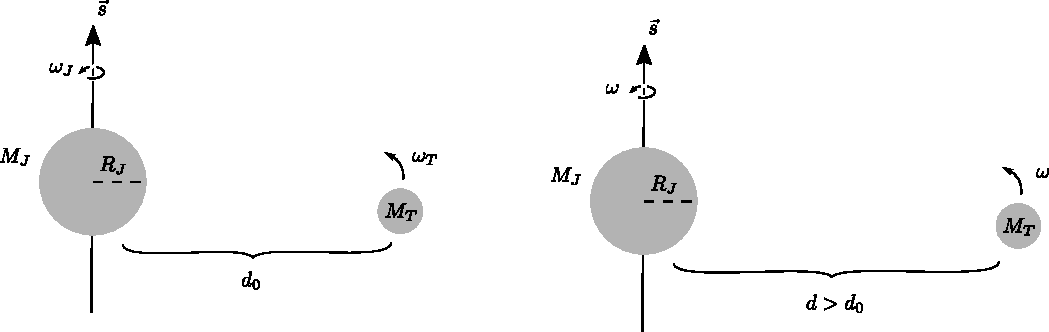
\includegraphics[width=\textwidth]{figures/earthmoon.pdf}
\end{figure}



Tunglið er að fjarlægjast jörðina um $\SI{4}{cm}$ á ári. Þetta veldur því að smátt og smátt fer jörðin að snúast hægar. Að lokum mun þetta leiða til þess að umferðartími tunglsins um jörðina verður sá sami og umferðartími jarðarinnar. Þetta fyrirbæri nefnist sjávarfallalæsing (e.~\textit{tidal locking}) og sjá má fyrirbærið hjá Karoni, tungli Plútós, sem svífur ávallt yfir sama punkti á Plútó. Í þessu dæmi munum við reyna að meta það hver lokasnúningshraði jarðarinnar verður og lokavegalengdina milli jarðarinnar og tunglsins. Látum massa jarðarinnar vera táknaðan með $M_J = \SI{5.97e24}{kg}$ og látum $M_T = \SI{7.35e22}{kg}$ tákna massa tunglsins. Látum geisla jarðarinnar vera táknaðan með $R_J = \SI{6.37e6}{m}$ Látum núverandi fjarlægð milli jarðarinnar og tunglsins vera táknaða með $d_0 = \SI{3.84e8}{m}$. Jörðin snýst um sjálfa sig, einn hring á einum degi. Veljum því snúningsás kerfisins í gegnum jörðina. Þá er hverfitregða kerfisins í dag gefin með:
\begin{align*}
    I_0 = I_J + I_T.
\end{align*}
Þar sem að
\begin{align*}
    I_J = \frac{2}{5}M_J R_J^2 = \SI{9.69e37}{kg.m^2} , \hspace{1cm} I_T = M_Td_0^2 = \SI{1.08e40}{kg.m^2}
\end{align*}
Við ályktum því að $I_0 \approx I_T = \SI{1.08e40}{kg.m^2} $. Við athugum síðan að jörðin snýst um sjálfa sig með hornhraða:
\begin{align*}
    \omega_J = \frac{2\pi}{T_J} = \frac{2\pi}{24 \cdot 60^2 \si{s}} = \SI{7.27e-5}{rad/s}.
\end{align*}
En hornhraði tunglsins í upphafi er gefinn með:
\begin{align*}
    \omega_T = \frac{2\pi}{27 \cdot 24 \cdot 60^2 \si{s}} = \SI{2.69e-6}{rad/s}. 
\end{align*}
Þar með höfum við að hverfiþungi kerfisins í upphafi er gefinn með:
\begin{align*}
    L_0 = I_J\omega_J + I_T \omega_T = \SI{7.04e33}{kg.m^2/s} + \SI{2.91e34}{kg.m^2/s} = \SI{3.62e34}{kg.m^2/s}.
\end{align*}
Þar sem að
\begin{align*}
    I = I_J + M_Td^2 \approx M_Td^2
\end{align*}
Því við sáum hér á undan að $I_J \ll I_T < M_Td^2$. 
En síðan er
\begin{align*}
    L = I \omega \approx M_Td^2\omega
\end{align*}
Hverfiþungavarðveislan gefur síðan að $L = L_0$. Við höfum síðan samkvæmt þriðja lögmáli Keplers að:
\begin{align*}
    \frac{d^3}{T^2} = \frac{GM_J}{4\pi^2}
\end{align*}
Sem við getum umritað þannig að:
\begin{align*}
    d^3\omega^2 = GM_J.
\end{align*}
Við höfum því jöfnuhneppi með tveimur óþekktum stærðum $\omega$ og $d$:
\begin{align*}
    \begin{cases}
    M_Td^2\omega = L_0, \\
    d^3\omega^2 = GM_J
    \end{cases}
\end{align*}
Hefjum fyrri jöfnuna í annað veldi og deilum í með seinni jöfnunni til að fá:
\begin{align*}
    M_T^2 d = \frac{M_T^2 d^4 \omega^2}{d^3 \omega^2} = \frac{L_0^2}{G M_J} \implies d  = \frac{L_0^2}{GM_J M_T^2} = \SI{6.09e8}{m} =  1,59d_0
\end{align*}
En þar með höfum við að:
\begin{align*}
    \omega = \frac{L_0}{M_Td^2} = \SI{1.33e-6}{rad/s}
\end{align*}
Sem myndi samsvara umferðartímanum $T = \frac{2\pi}{\omega} = \SI{4.73e6}{s} = \SI{55}{dagar}$. \\

Við skulum núna velta fyrir okkur ástæðunni sem liggur að baki þessu. Það er yfirleitt nefnt í umfjöllun um flóð og fjöru að tunglið sé helsta orsök sjávarfalla. Sólin leggur hinsvegar einnig framlag til málsins og því fáum við stundum stórstreymi þegar flóðkraftar tungls og sólar leggjast saman vegna afstöðu tunglsins miðað við jörðina og sólina og hinsvegar smástreymi þegar flóðkraftar tungls og sólar vinna gegn hvorum öðrum. Eitt sem gleymist reglulega í umræðunni er að þyngdarlögmálskraftur sólarinnar er sterkari heldur en þyngdarlögmálskraftur tunglsins á yfirborði jarðarinnar. Við athugum nefnilega að hröðunin sem hlutir á yfirborði jarðarinnar finna fyrir vegna sólarinnar er gefin með:
\begin{align*}
    a_S = \frac{GM_S}{R_S^2} = \frac{\SI{6.67e-11}{m^3/(kg.s^2)} \cdot \SI{1.99e30}{kg}}{(\SI{1.50e11}{m})^2} = \SI{5.93e-3}{m/s^2}
\end{align*}
Hinsvegar er hröðunin sem hlutir á yfirborði jarðarinnar finna fyrir vegna tunglsins gefin með:
\begin{align*}
    a_T = \frac{GM_T}{d_0^2} = \frac{\SI{6.67e-11}{m^3/(kg.s^2)} \cdot \SI{1.99e30}{kg}}{(\SI{3.84e8}{m})^2} = \SI{3.32e-5}{m/s^2} < a_S
\end{align*}
Við sjáum því að sólin togar fastar heldur en tunglið í hluti á yfirborði jarðarinnar. Við sjáum reyndar að: $a_S/a_T = 179$ svo sólin togar 179 sinnum fastar í okkur á yfirborði jarðarinnar heldur en tunglið. Hvernig stendur þá á því að framlag tunglsins til sjávarfalla sé meira heldur en sólarinnar? Við skulum skoða einfalt líkan til þess að reyna að varpa ljósi á þetta skrítna fyrirbrigði. Við getum nú farið að tala um sýndarkrafta. Flóðkrafturinn er sýndarkraftur. Hann er í rauninni bara þyngdarlögmálskrafturinn í dulbúningi. Okkur finnst eins og að þetta sé sjálfstæður kraftur því við erum í viðmiðunarkerfi sem finnur fyrir hröðun (vegna þyngarlögmálskraftins). Við þurfum því að hugsa um afstæða hröðun hlutarins miðað við viðmiðunarkerfið sem við erum í. Jörðin finnur fyrir þyngdarlögmálskrafti vegna sólarinnar (og tunglsins). Sá kraftur verkar á massamiðju jarðarinnar. Við sjáum þá að:
\begin{align*}
    ma = m\left(a_{\text{sýndar}} + a_J \right) = \frac{GM_Sm}{(R_S-R_J)^2}
\end{align*}
En við vitum að $a_J = \frac{GM_S}{R_S^2}$ svo við fáum að:
\begin{align*}
    F_{\text{sýndar}} = ma_{\text{sýndar}} = \frac{GM_Sm}{(R_S-R_J)^2} - \frac{GM_Sm}{R_S^2} = \frac{GM_Sm}{R_S^2}\left( \left(1 - \frac{R_J}{R_S} \right)^{-2} - 1 \right) \approx \frac{GM_Sm}{R_S^2}\left(1 + \frac{2R_J}{R_S} - 1 \right) = \frac{2GM_SmR_J}{R_S^3}.
\end{align*}
En þar með getum við athugað hvort hefur meira áhrif á sjávarföll, tunglið eða sólin. Við athugum að:
\begin{align*}
    \frac{F_{\text{flóð, tungl}}}{F_{\text{flóð, sól}}} = \frac{\frac{2GM_TmR_J}{R_T^3}}{\frac{2GM_SmR_J}{R_S^3}} = \left(\frac{M_T}{M_S}\right) \cdot \left(\frac{R_S}{R_T}\right)^3 = \left( \frac{\SI{7.35e22}{kg}}{\SI{1.99e30}{kg}} \right) \cdot \left( \frac{\SI{1.50e11}{m}}{\SI{3.84e8}{m}} \right)^3 = \SI{2.20}{} 
\end{align*}
Svo við ályktum að tunglið hefur um það bil tvisvar sinnum meiri áhrif á flóðkraftana. Við getum líka gefið gróft mat á hversu stór hæðarbreytingin er vegna flóðkraftanna. Við byrjum á því að athuga að stöðuorka flóðkraftsins er gefin með:
\begin{align*}
    U_{flóð} = -\frac{GM_Sm}{R_S^3}r^2
\end{align*}
þar sem að $r$ er fjarlægðin að miðju jarðarinnar. Við sjáum þá að á yfirborði jarðarinnar, þar sem $r = R_J$, þá höfum við:
\begin{align*}
    mgh = \frac{GM_SmR_J^2}{R_S^3} \implies h_S = \frac{M_S}{M_J} \frac{R_J^4}{R_S^3} = \SI{0.163}{m}
\end{align*}
og fyrir tunglið fæst eins að:
\begin{align*}
    h_T = \frac{M_T}{M_J} \frac{R_J^4}{R_T^3} = \SI{0.358}{m}
\end{align*}
Við höfum þá einmitt enn að $\frac{h_T}{h_S} = \SI{2.20}{}$. Í heildina sjáum við að flóðbylgjur hafa um það bil mesta hæð $h = h_S + h_T = \SI{0.521}{m}$. 

\end{comment}


\newpage

\section{Dæmi}

\begin{enumerate}[label = \textbf{Dæmi \thechapter.\arabic*.}]

\subsection*{Hornstaða, hornhraði og hornhröðun}

\item \textit{(RK 12.1.)} BOSCH Höggborvélin PSB 700-2RE (sem fæst í BYKO) hefur hámarkssnúningshraða $\SI{3000}{snú/mín}$. Það tekur borvélina $\SI{0.75}{s}$ að ná þeim snúningshraða úr kyrrstöðu.
\begin{enumerate}[label = \textbf{(\alph*)}]
    \item Hver er meðalhornhröðun borsins á þeim tíma?
    \item Hversu marga snúninga snýst borinn á þeim tíma sem það tekur hann að ná hámarkssnúningshraða?
\end{enumerate}

\item \textit{(RK 12.3.)} Loftviftur eru snjöll leið til að dreifa varma og koma hreyfingu á loft. Lítum á iðnaðarloftviftu sem hefur \SI{142}{cm} þvermál og snýst með hraða $\SI{250}{snú/mín}$. Hugsum okkur að við slökkvum á viftunni. Þá tekur það viftuna $\SI{60}{s}$ að stöðvast.

\begin{enumerate}[label = \textbf{(\alph*)}]
    \item Hver er meðalhornhröðun viftunnar frá því að slökkt er á viftunni og þar til viftan hefur stöðvast.
    \item Hver er hornhraði viftunnar, $\SI{18}{s}$, eftir að það hefur verið slökkt á viftunni?
    \item Hversu marga snúninga snýst viftan áður en að hún stöðvast?
\end{enumerate}

\item Geisladiskur varðveitir tónlist sem röð smárra dælda í yfirborði disksins $\SI{1.0e-7}{m}$ að dýpt. Dældunum er raðað eftir rás sem er eins og spírall að lögun frá innri að ytri brún disksins. Innri geisli spíralsins er $\SI{25}{mm}$ en sá ytri er $\SI{58}{mm}$. Þegar diskur er spilaður er rásin skönnuð með föstum línulegum hraða sem er $\SI{1.25}{m/s}$.

\begin{enumerate}[label = \textbf{(\alph*)}]
    \item Hver er hornhraði geisladisksins þegar verið er að lesa innsta hluta rásarinnar? En þegar ysti hluti rásarinnar er lesinn?
    
    \item Lengsti afspilunartími geisladisks er $\SI{74}{mín}$. Hver er lengd rásar í þannig geisladiski ef við réttum úr henni og gerðum úr henni rás eftir beinni línu?
\end{enumerate}


\begin{comment}




\item Flestir plötuspilarar hafa tvær hraðastillingar, annars vegar $33 \frac{1}{3}$ snúningar á mínútu og hinsvegar $45$ snúningar á mínútu. Fyrri stillingin er notuð til að spila stærri plötur sem hafa geisla $r_A = \SI{15.3}{cm}$ en seinni stillingin er notuð til að spila litlar plötur sem hafa geisla $r_B = \SI{8.9}{cm}$.

\begin{enumerate}[label = \textbf{(\alph*)}]
    \item Ákvarðið hornhraða plötuspilarans á hvorri stillingu fyrir sig, þ.e.~ákvarðið $\omega_A$ og $\omega_B$.
    \item Skoðum núna fyrri hraðastillinguna aðeins nánar. Innsta röndin á vínýl-plötu sem nál plötuspilarans getur lesið hefur geisla $\text{r}_0 = \SI{6.0}{cm}$ og ysta röndin hefur geisla $\text{r}_1 = \SI{14.6}{cm}$. Hver er línulegur hraði nálarinnar innst, $v_0$, og yst, $v_1$, á plötunni?
    \item Afspilunartími (á einni hlið) á dæmigerðri vínýl-plötu á fyrri hraðastillingunni er $\SI{22}{\text{mínútur}}$. Bilið á milli ráka plötunnar er $d = \SI{65}{\mu m}$. Þar sem að hornhraði plötunnar er fastur þá snýst platan einn hring á föstum tíma sem þýðir að nálin færist alltaf vegalengd $d$ inn í áttina að miðju plötunnar með föstum, miðlægum hraða. Ákvarðið þennan miðlæga hraða.
\end{enumerate}
\end{comment}

\subsection*{Massamiðja}



\item \textit{(RK 12.5.)} Jörðin hefur massa $M_J = \SI{5.97e24}{kg}$, tunglið hefur massa $M_T = \SI{7.35e22}{kg}$ og sólin hefur massa $M_S = \SI{1.99e30}{kg}$. Meðalfjarlægðin milli jarðarinnar og tunglsins er $d = \SI{3.84e8}{m}$ og meðalfjarlægðin milli jarðarinnar og sólarinnar er $R = \SI{1}{AU} = \SI{1.50e11}{m}$. Hugsum okkur að Sólin, Jörðin og Tunglið liggi í beinni línu (í þessari röð). Veljum hnitakerfi þar sem að sólin er í $x = 0$, jörðin er í $x = R$ og tunglið er í $x = R+d$.

\begin{figure}[H]
    \centering
    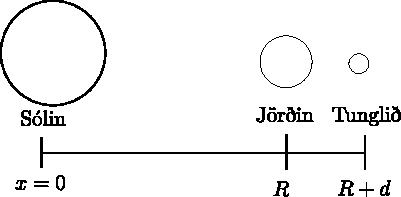
\includegraphics{figures/soljordtungl.pdf}
\end{figure}

\begin{enumerate}[label = \textbf{(\alph*)}]
    \item Ákvarðið massamiðju jarðarinnar og tunglsins.
    \item Ákvarðið massamiðju sólarinnar og jarðarinnar.
    \item Ákvarðið massamiðju kerfisins.
\end{enumerate}


\begin{minipage}{\linewidth}

\begin{wrapfigure}{r}{1.2in}
\vspace{-3cm}
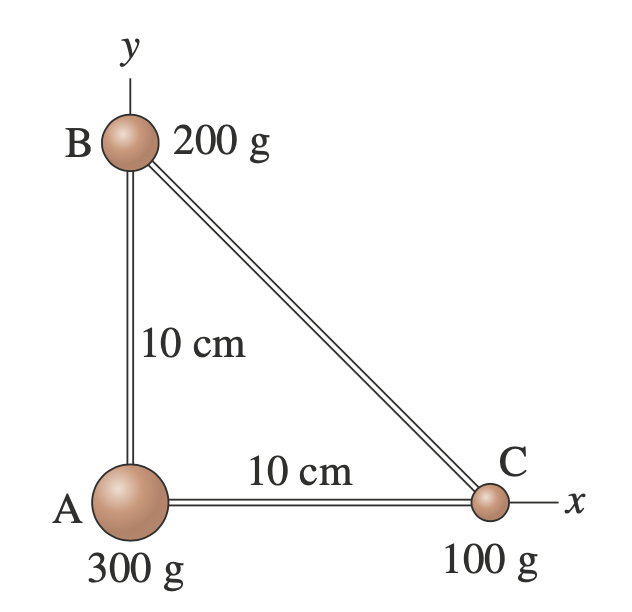
\includegraphics[width=1.85in]{images/cmbert.png}
\end{wrapfigure}

\item \textit{(RK 12.6.)} Ákvarðið massamiðju eftirfarandi kerfisins hér til hægri þar sem að punktmassarnir þrír eru tengdir með massalausum vírum og punkturinn $A$ er staðsettur í upphafspunkti hnitakerfisins.

\end{minipage}


\newpage

\subsection*{Hverfitregður og snúningsásar}

\item Finnið hverfitregður eftirfarandi hluta:

\vspace{0.3cm}

\begin{figure}[h]
    \centering
    \begin{subfigure}[t]{0.4\textwidth}
        \centering
        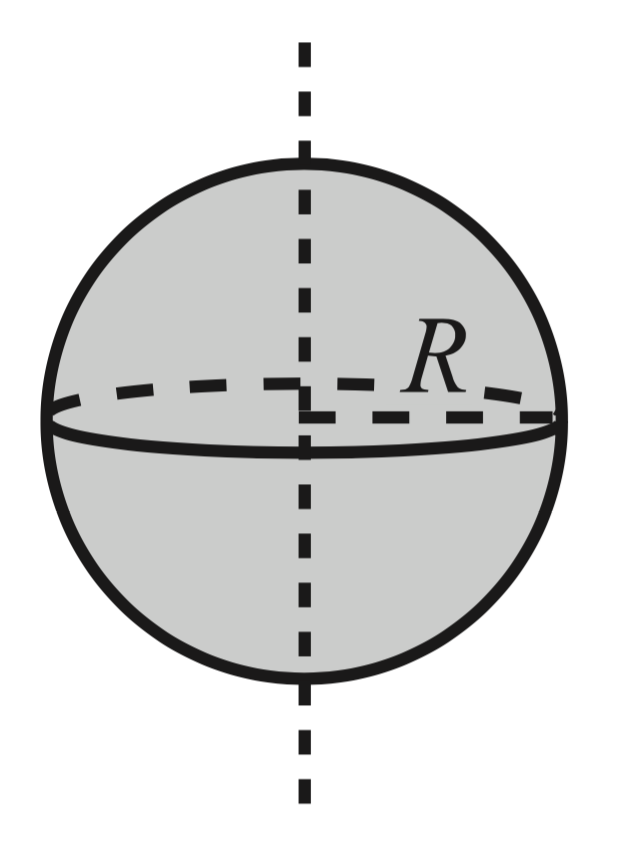
\includegraphics[height=1.3in]{images/gkula.png}
        \caption{Gegnheil kúla með massa $m$ og geisla $R$ miðað við ás gegnum miðju kúlunnar.}
    \end{subfigure}
    ~ 
    \begin{subfigure}[t]{0.4\textwidth}
        \centering
        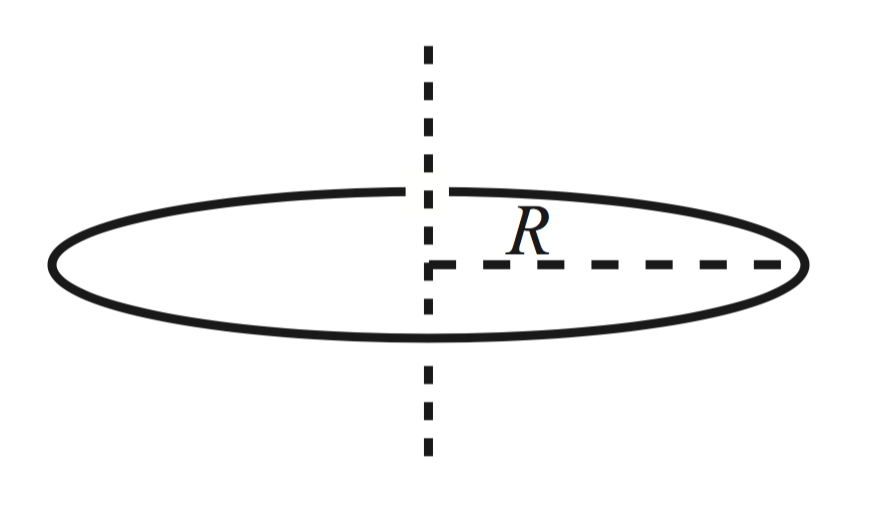
\includegraphics[height=1.1in]{images/gjord.png}
        \caption{Gjörð með massa $m$ og geisla $R$ miðað við ás gegnum miðjuna, hornrétt á flötinn.}
    \end{subfigure}
    ~ 
    \begin{subfigure}[t]{0.4\textwidth}
        \centering
        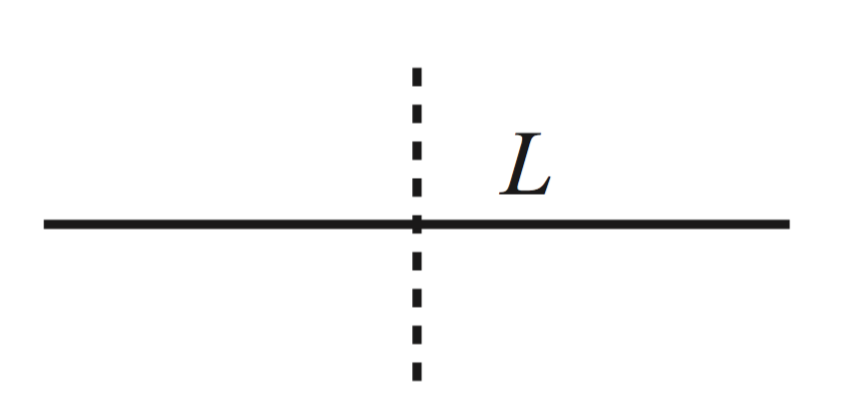
\includegraphics[height=0.8in]{images/stong.png}
        \caption{Stöng með massa $m$ af lengd $L$ miðað við ás gegnum miðju stangarinnar.}
    \end{subfigure}
    ~ 
    \begin{subfigure}[t]{0.4\textwidth}
        \centering
        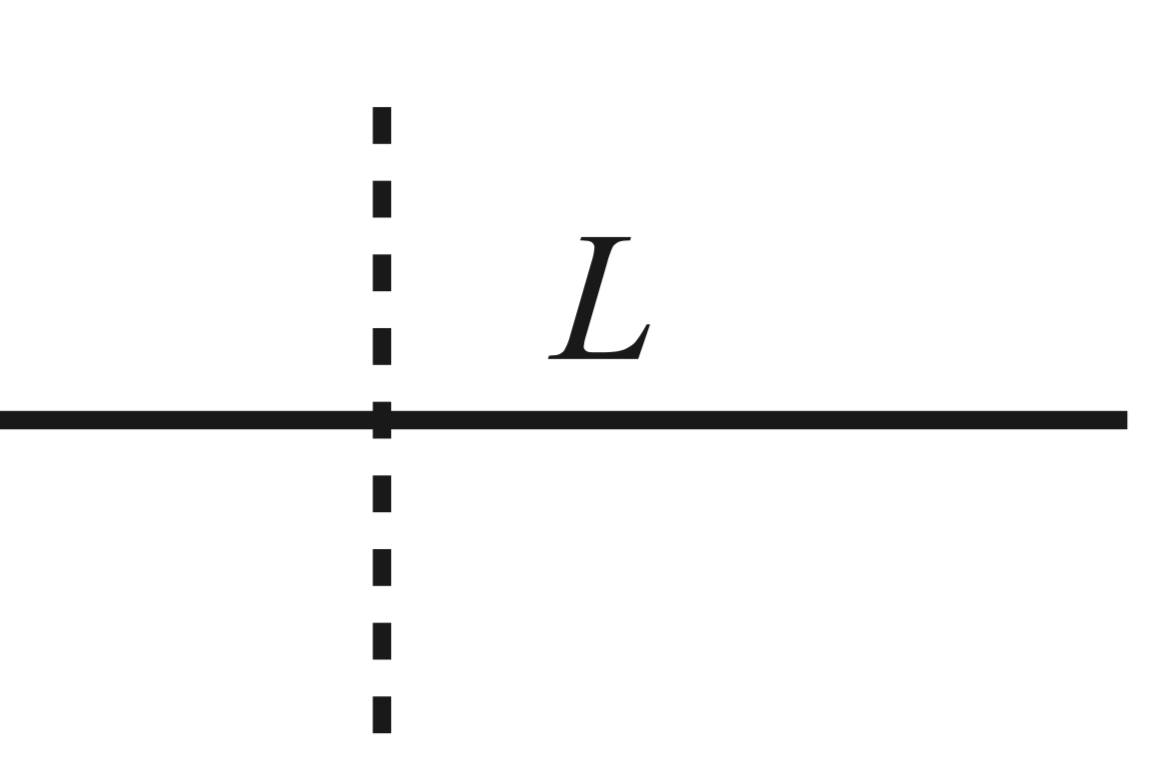
\includegraphics[height=1in]{images/steinerston.png}
        \caption{Stöng með massa $m$ af lengd $L$ miðað við ás í fjarlægð $L/3$ frá enda stangarinnar.}
    \end{subfigure}
\end{figure}

\begin{minipage}{\linewidth}

\begin{wrapfigure}{r}{1.5in}
\vspace{-1cm}
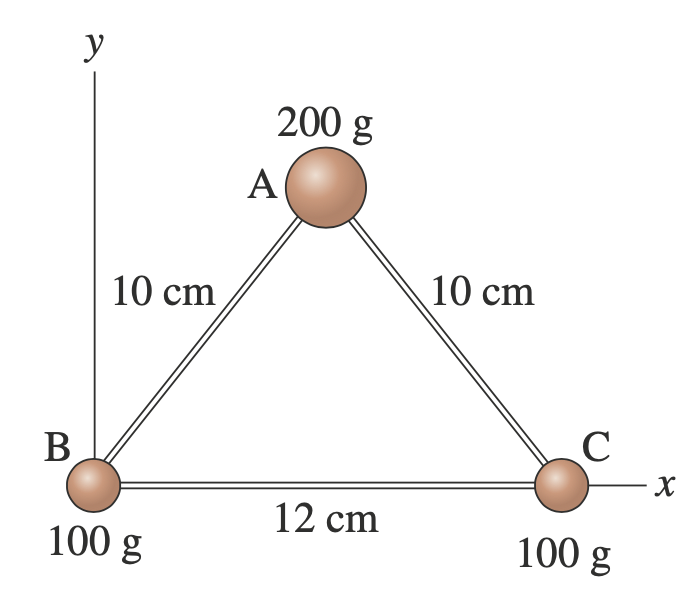
\includegraphics[width=2in]{images/inertiarot2.png}
\end{wrapfigure}

\item \textit{(RK 12.15.)} Massarnir þrír sem sjást á myndinni hér til hægri eru festir saman með massalausum vírum.

\begin{enumerate}[label = \textbf{(\alph*)}]
    \item Ákvarðið massamiðju kerfisins.
    \item Ákvarðið hverfitregðu kerfisins um ás sem liggur inn í blaðið í gegnum punktinn A.
    \item Ákvarðið hverfitregðu kerfisins um ás sem liggur í gegnum punktana B og C.
\end{enumerate}

\end{minipage}

\item \textit{(RK 12.17.)} Brunavarnarhurð nokkur hefur massa $m = \SI{20}{kg}$, hæð $h = \SI{210}{cm}$, breidd $b = \SI{84}{cm}$ og þykkt $þ = \SI{10}{cm}$.
\begin{enumerate}[label = \textbf{(\alph*)}]
    \item Hver er hverfitregða hurðarinnar um lóðréttan ás sem liggur í gegnum hjarirnar?
    \item Hver er hverfitregða hurðarinnar um láréttan ás sem liggur þvert á hurðina í hæð $y = \SI{12}{cm}$?
\end{enumerate}


\begin{minipage}{\linewidth}

\begin{wrapfigure}{r}{2.4in}
\vspace{-0.75cm}
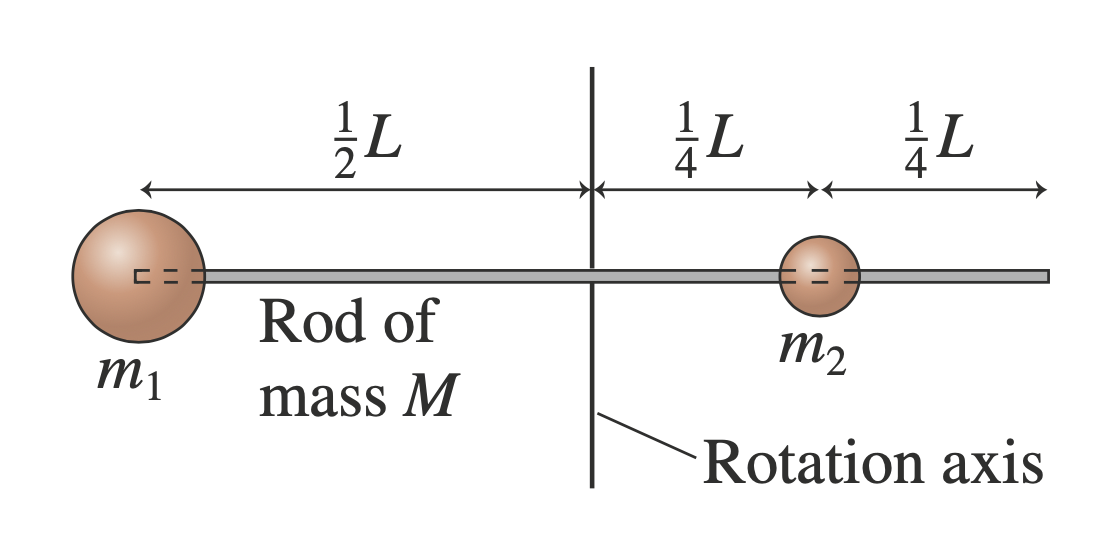
\includegraphics[width=3in]{images/gone.png}
\end{wrapfigure}

\item \textit{(RK 12.51)} Á myndinni hér fyrir neðan er kúla með massa $m_1 = \SI{2.0}{kg}$ fest við stöng með massa $M = \SI{3.5}{kg}$ sem hefur lengd $L = \SI{1.2}{m}$. Í fjarlægð $\frac{1}{4}L = \SI{30}{cm}$ frá enda stangarinnar er kúla með massa $m_2 = \SI{1.0}{kg}$.

\begin{enumerate}[label = \textbf{(\alph*)}]
    \item Ákvarðið hverfitregðu kerfisins um miðju stangarinnar.
    \item Ákvarðið massamiðju kerfisins.
    \item Ákvarðið hverfitregðu kerfisins um snúningsás sem liggur í gegnum massamiðju kerfisins.
\end{enumerate}

\end{minipage}

\item Uppbygging jarðarinnar er þannig að hún samanstendur kjarna með geisla $r_k = \SI{3500}{km}$ sem hefur eðlismassa $\rho_k = \SI{1.3e4}{kg/m^3}$. Utan á kjarnanum liggur síðan möttullinn og jarðskorpan sem hafa eðlismassa $\rho_m = \SI{4.0e3}{kg/m^3}$. Geisli jarðarinnar er $r_m = \SI{6400}{km}$. Hver er eðlismassi jarðarinnar, $I_J$, um ás sem liggur í gegnum miðju hennar?





\subsection*{Kraftvægi}

\begin{minipage}{\linewidth}

\begin{wrapfigure}{r}{1.5in}
\vspace{-0.755cm}
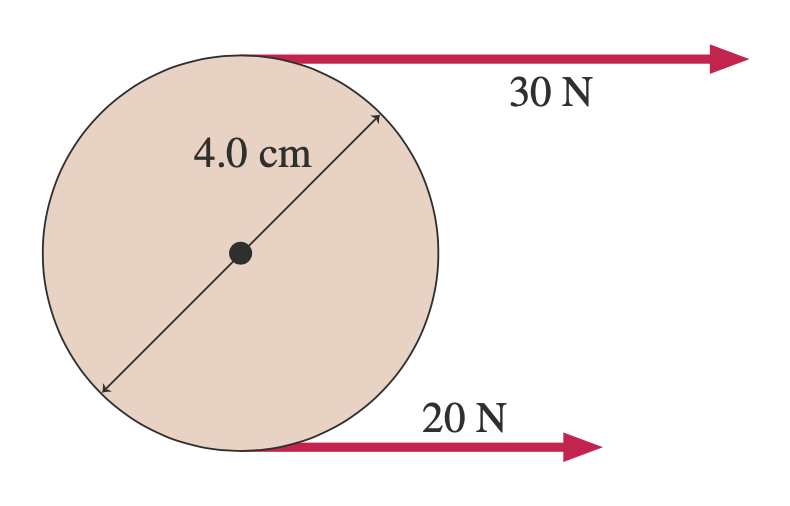
\includegraphics[width=2in]{images/torque1.png}
\end{wrapfigure}

\item \textit{(RK 12.18.)} Lítum á gegnheila sívalinginn hér til hægri sem hefur massa $m = \SI{1.5}{kg}$ og geisla $r = \SI{4.0}{cm}$.

\begin{enumerate}[label = \textbf{(\alph*)}]
    \item Ákvarðið kraftvægið, $\tau$, sem verkar á sívalinginn um ás sem liggur út úr blaðinu.
    \item Notið $2.$ lögmál Newtons fyrir snúninga til þess að ákvarða hornhröðun gegnheila sívalingsins.
\end{enumerate}

\end{minipage}

\vspace{0.5cm}

\begin{minipage}{\linewidth}

\begin{wrapfigure}{r}{1.2in}
\vspace{-0.755cm}
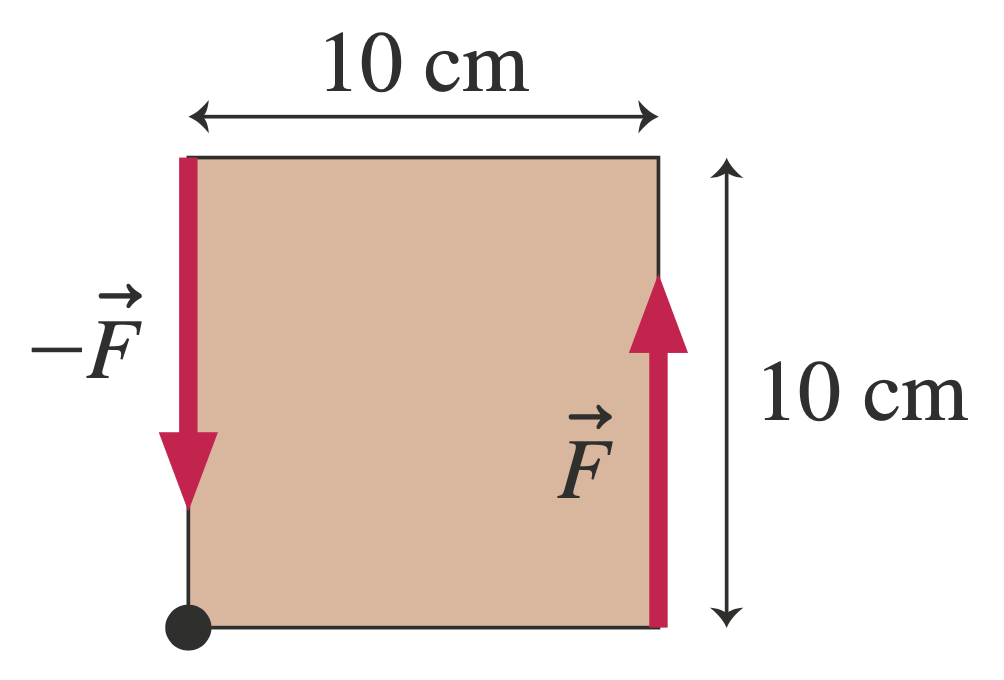
\includegraphics[width=2in]{images/torque2.png}
\end{wrapfigure}

\item \textit{(RK 12.19.)} Lítum á myndina hér til hægri. Þar má sjá gegnheilan rétthyrning sem hefur hliðarlengdir $\ell = \SI{10}{cm}$ og massa $m = \SI{150}{g}$. Krafti $F = \SI{50}{N}$ er beitt beint upp á neðra hægra horn rétthyrningsins. Á sama tíma er jafnstórum (en gagnverkandi) krafti beitt beint niður á efra, vinstra horn rétthyrningsins.

\begin{enumerate}[label = \textbf{(\alph*)}]
    \item Ákvarðið kraftvægið um ás sem liggur út úr blaðinu í gegnum neðri, vinstri hornpunkt rétthyrningsins.
    \item Ákvarðið kraftvægið um massamiðju rétthyrningsins.
\end{enumerate}

\end{minipage}

\vspace{0.5cm}

\begin{minipage}{\linewidth}

\begin{wrapfigure}{r}{1.2in}
\vspace{-1cm}
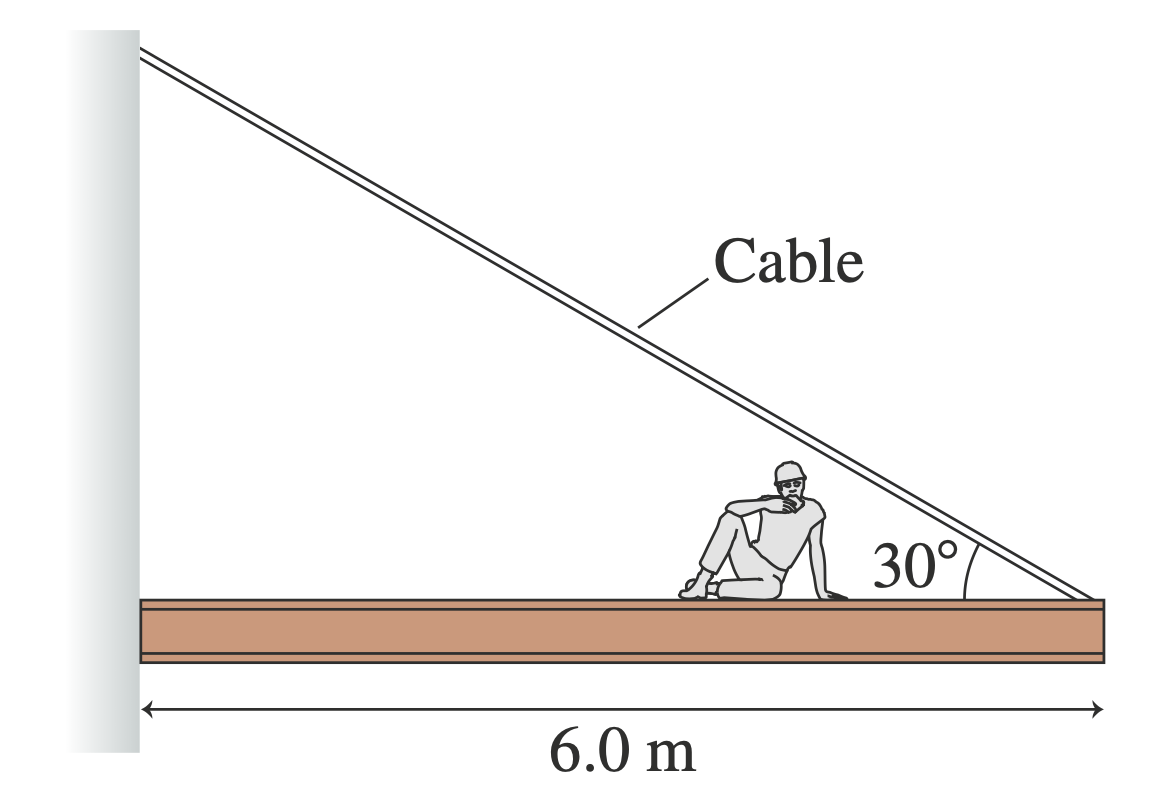
\includegraphics[width=1.85in]{images/construct.png}
\end{wrapfigure}

\item \textit{(RK 12.59.)} Iðnaðarmaður með massa $m = \SI{80}{kg}$ situr (að borða hádegismatinn sinn) í $\SI{2.0}{m}$ fjarlægð frá enda stálbjálksins (sem hefur heildarlengdina $\SI{6.0}{m}$). Massi stálbjálkans er $\SI{1450}{kg}$. Hver er togkrafturinn í vírnum sem heldur bjálkanum og iðnarðarmanninum uppi?
\end{minipage}

\vspace{0.5cm}

\begin{minipage}{\linewidth}

\begin{wrapfigure}{r}{1.2in}
\vspace{0.5cm}
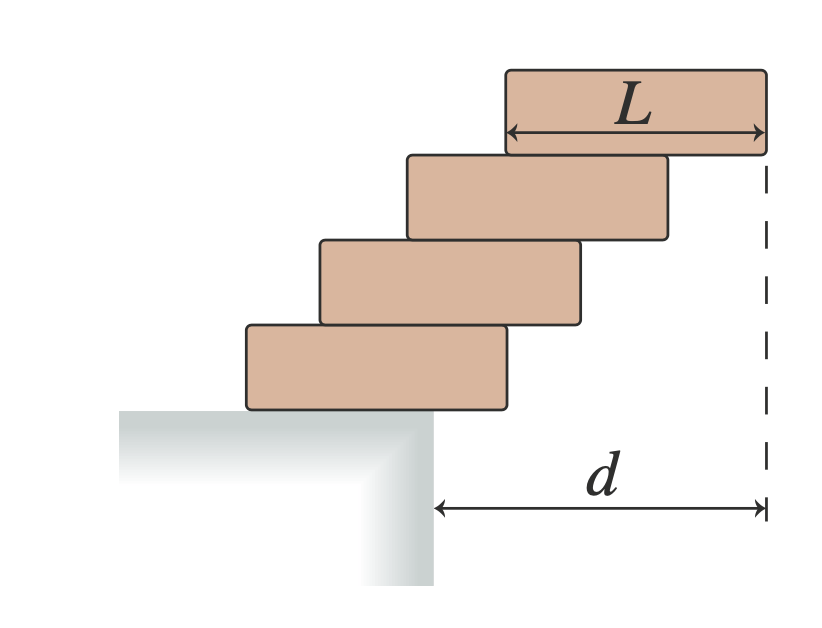
\includegraphics[width=1.85in]{images/restacks.png}
\end{wrapfigure}

\item \textit{(RK 12.61.)} Þið eruð að taka þátt í framkvæmdakeppni framhaldsskólanna. Þið hafið fengið $4$ eins kubba með massa $m$ og lengd $L$. Markmiðið ykkar er að reyna að stafla kubbunum þannig að þeir geti staðið eins langt fram af borðinu um vegalengd $d$ eins og sést á mynd hér til hægri. Hvert er stærsta gildið á $d$?

\vspace{0.5cm}


\item Fyrir utan bifreiðaverkstæði Pálmfríðar hengur stórt auglýsingarskilti sem hefur massann $\SI{21.9}{kg}$. Skiltið er fest með vír í einsleita bómu af lengd $\SI{1.70}{m}$. Bóman hefur massa $\SI{15.8}{kg}$. Þar að auki er vír festur við bómuna $\SI{1.35}{m}$ frá enda veggjarins. Sá vír myndar $\SI{35}{\degree}$ horn miðað við lárétt.  Finnið togkraftana í báðum vírunum ásamt lóðréttum og láréttum kröftum sem hjarir bómunnar verka með á vegginn.
\end{minipage}

\begin{figure}[H]
    \centering
    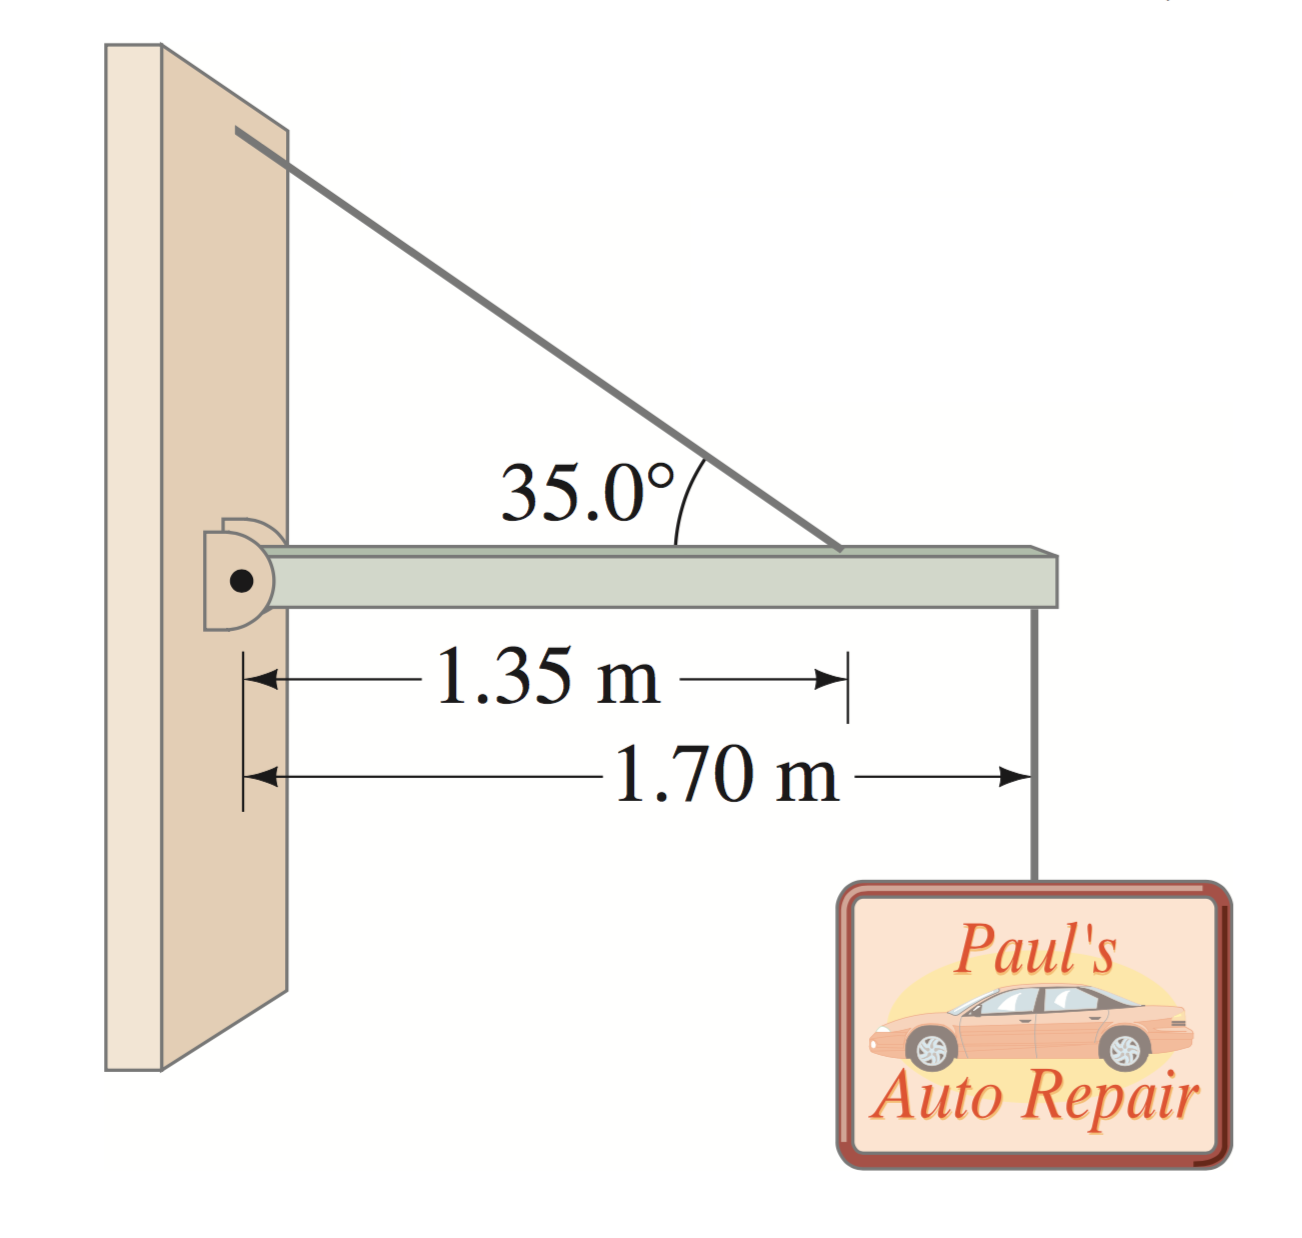
\includegraphics[scale = 0.3]{images/anna.png}
\end{figure}


\begin{minipage}{\linewidth}

\begin{wrapfigure}{r}{1.1in}
\vspace{-1.4cm}
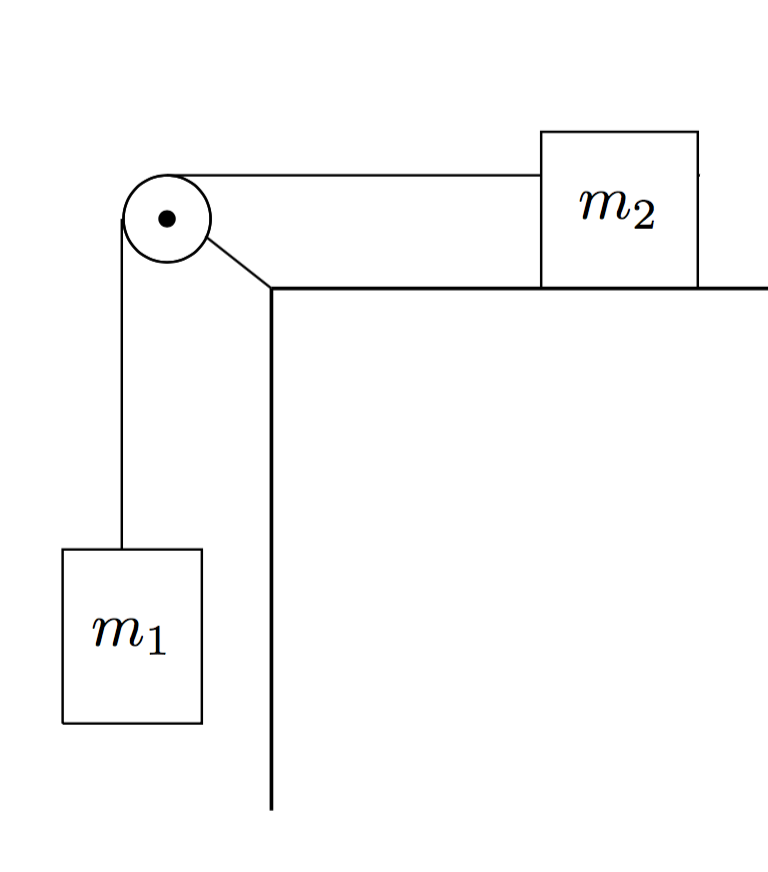
\includegraphics[width=1.75in]{images/trissa.png}
\end{wrapfigure}
\item Kassi með massa $m_2 = \SI{11}{kg}$ liggur á láréttum fleti með núningsstuðul $\mu = 0.3$. Kassinn er festur með vír við annan kassa með massa $m_1 = \SI{18}{kg}$ yfir trissu með massa $m = \SI{3.1}{kg}$ og geisla $r = \SI{0.14}{m}$.
\begin{enumerate}
    \item Finnið hornhröðun trissunnar um ás sem liggur í gegnum miðju trissunnar út úr blaðinu.
    \item Finnið hröðun kerfisins eftir að því er sleppt úr kyrrstöðu.
\end{enumerate}
\end{minipage}

\vspace{0.5cm}

\begin{minipage}{\linewidth}
\begin{wrapfigure}{r}{1.5in}
\vspace{-0.25cm}
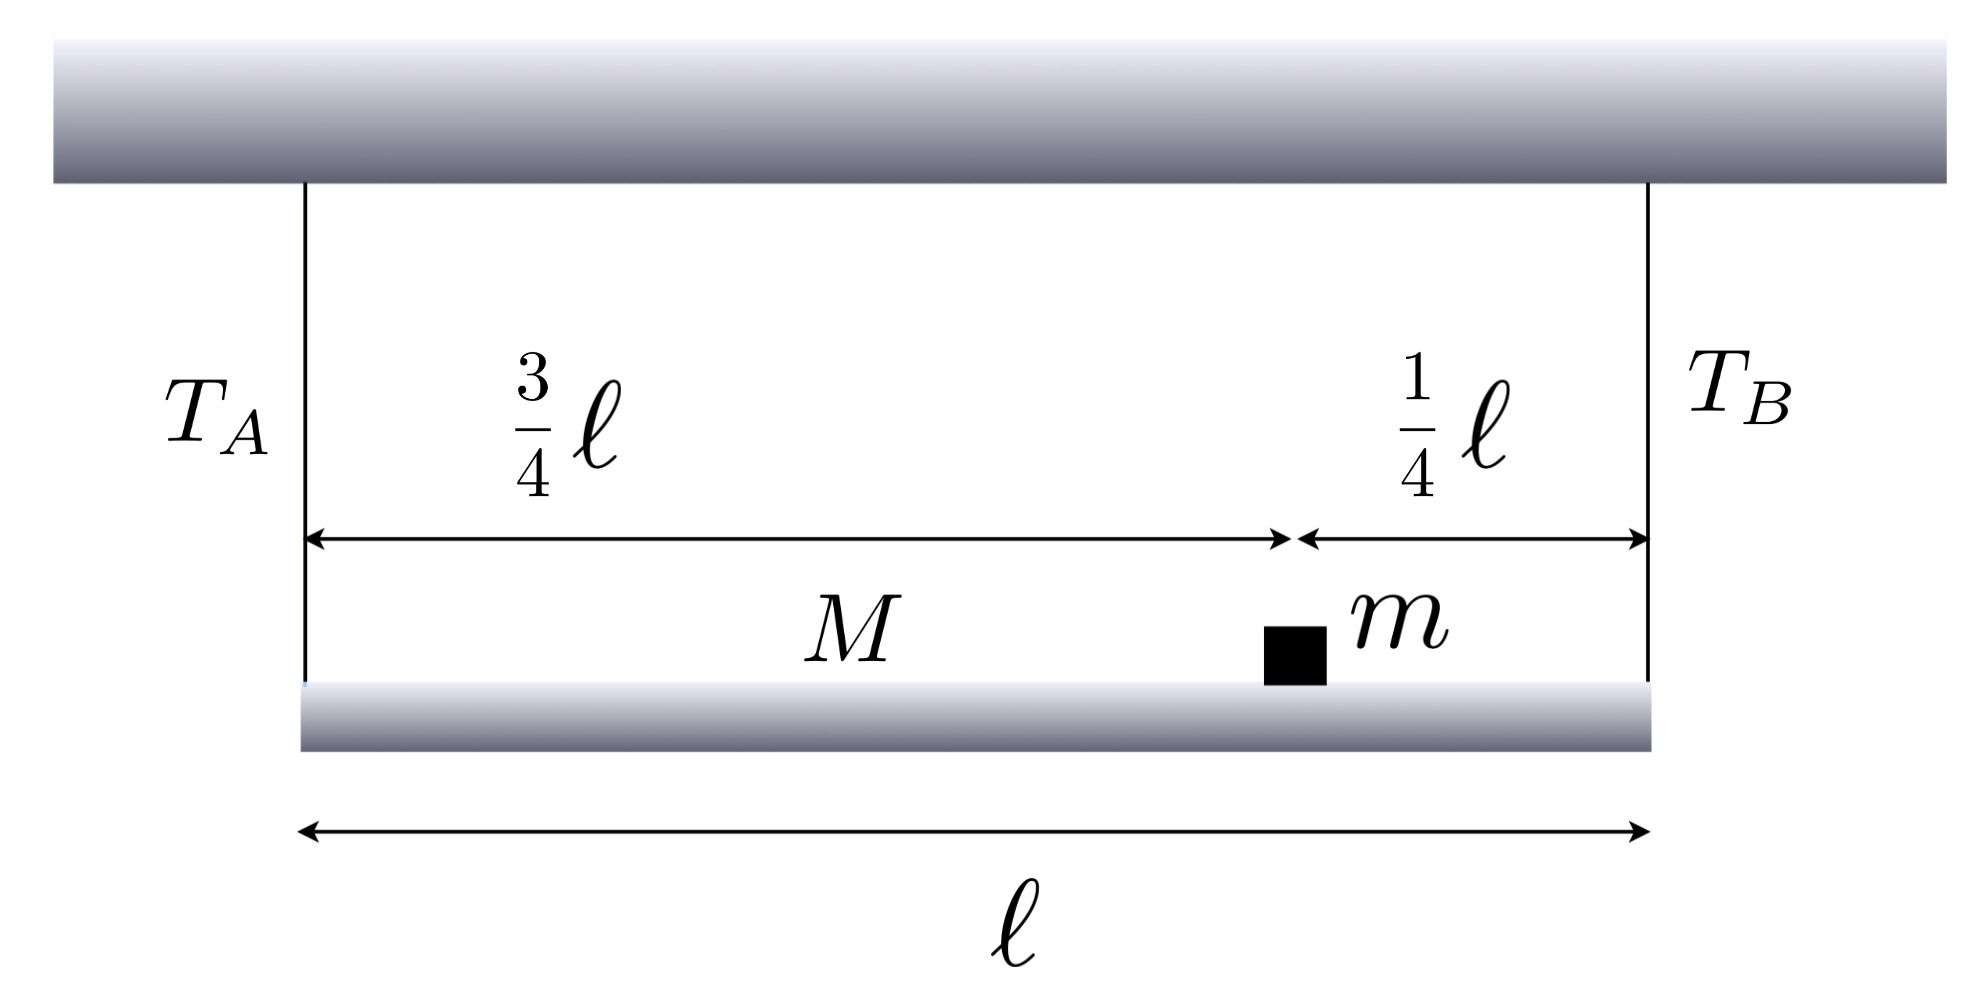
\includegraphics[width=2.3in]{images/bjalkens.png}
\end{wrapfigure}

\item Einsleitum bjálka með massa $M = \SI{16.8}{kg}$ og af lengd $\ell = \SI{2.0}{m}$ er haldið uppi af tveimur eins vírum með togkröftum $T_A$ og $T_B$. Lítill kubbur með massa $m = \SI{5.2}{kg}$ situr á bitanum í fjarlægð $\frac{1}{4}\ell$ frá öðrum enda bjálkans. 
\end{minipage}
\vspace{0.1cm}
\begin{enumerate}[label = \textbf{(\alph*)}]
    \item Skrifið niður kraftajöfnur og kraftvægisjöfnur.
    \item Ákvarðið togkraftana $T_A$ og $T_B$ í vírunum.
    \item Nú klippum við vírinn sem hefur togkraft $T_B$. Hver verður hornhröðun \\ kerfisins rétt eftir að klippt hefur verið á vírinn? Um hvaða snúningsás snýst kerfið?
\end{enumerate}

\vspace{0.5cm}

\begin{minipage}{\linewidth}

\begin{wrapfigure}{r}{1.9in}
\vspace{-0.5cm}
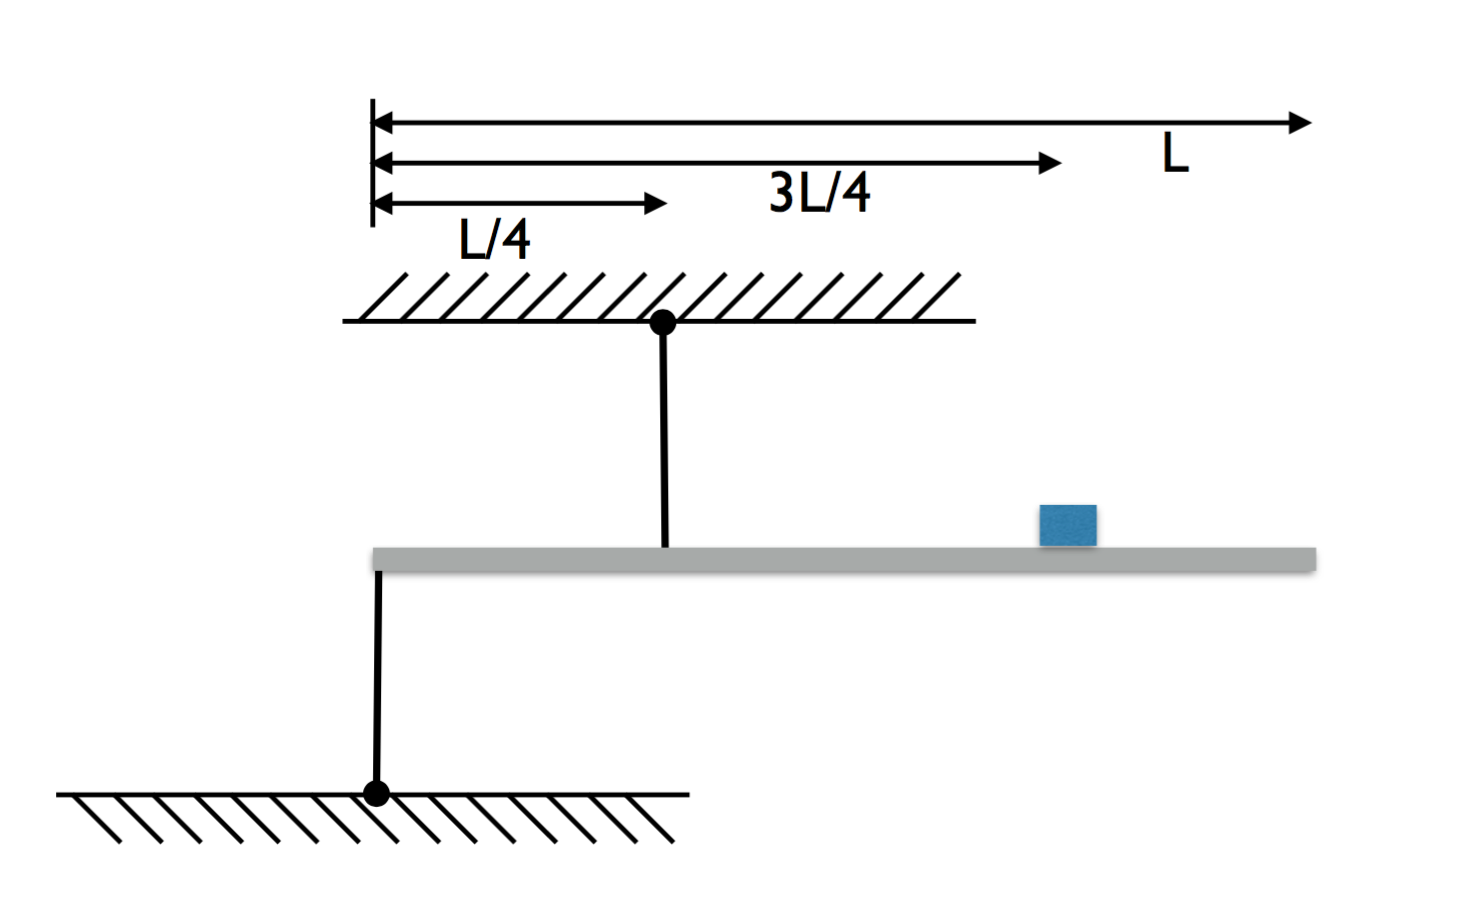
\includegraphics[width=2.65in]{images/jafnvaegi.png}
\end{wrapfigure}

\item Einsleitum planka með massa $m_p = \SI{10}{kg}$ og lengd $L = \SI{2.0}{m}$ er haldið í jafnvægi með tveimur massalausum vírum. Á plankanum stendur þar að auki líill kassi með massa $m_k = \SI{5}{kg}$.
\end{minipage}

\begin{enumerate}[label = \textbf{(\alph*)}]
    \item Finnið togkraftinn $T_1$ í vírnum sem festur er niður í gólf.
    
    \item Finnið togkraftinn $T_2$ í vírnum sem festur er upp í loft.
    
    \item Nú klippum við vírinn sem festur er niður í gólf. \\ Finnið hornhröðun plankans
    rétt eftir að vírinn hefur verið klipptur.
    
\end{enumerate}

\vspace{0.75cm}


\begin{minipage}{\linewidth}

\begin{wrapfigure}{r}{1.2in}
\vspace{-0.75cm}
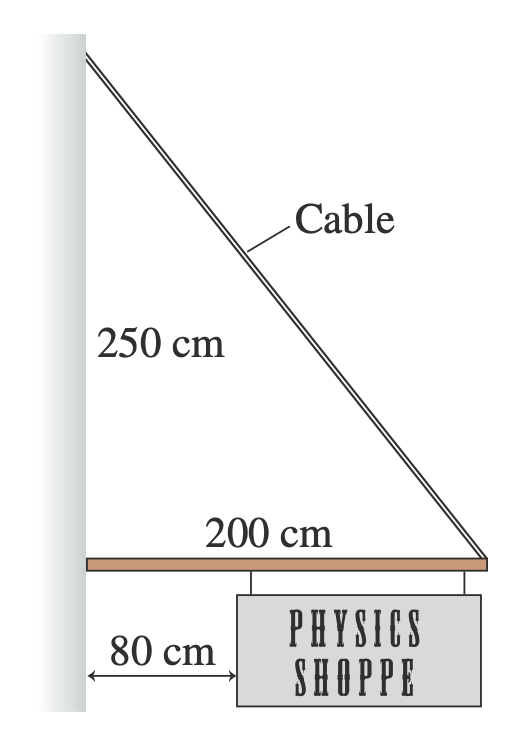
\includegraphics[width=1.85in]{images/vir.png}
\end{wrapfigure}

\item \textit{(RK 12.62.)} Skilti af lengd $\SI{120}{cm}$ hengur úr $\SI{5.0}{kg}$ bómu af lengd $\SI{200}{cm}$. Massalaus vír er festur við enda bómunnar í vegginn $\SI{250}{cm}$ ofar eins og sjá má á myndinni hér til hægri. Hver er mesta þyngdin sem skiltið má hafa ef vírinn slitnar þegar togkrafturinn í strengnum fer yfir $\SI{300}{N}$?

\vspace{0.5cm}

\item \textit{(RK 12.86.)} Tveir massar, $m_1 = \SI{4.0}{kg}$ og $m_2 = \SI{2.0}{kg}$ eru festir með massalausu bandi yfir trissu (sem er hvorki núninglaus né massalaus!) með geisla $r = \SI{12}{cm}$ og massa $m = \SI{2.0}{kg}$. Vægi núningskraftsins er $\SI{0.50}{Nm}$ um hjólás trissunar (inn í blaðið). Hversu langur tími, $t$, líður frá því að kerfinu er sleppt úr kyrrstöðu og þar til að stóri massinn, $m_1$, lendir á jörðinni, $\SI{1.0}{m}$ neðar?
\end{minipage}

\begin{figure}[H]
    \centering
    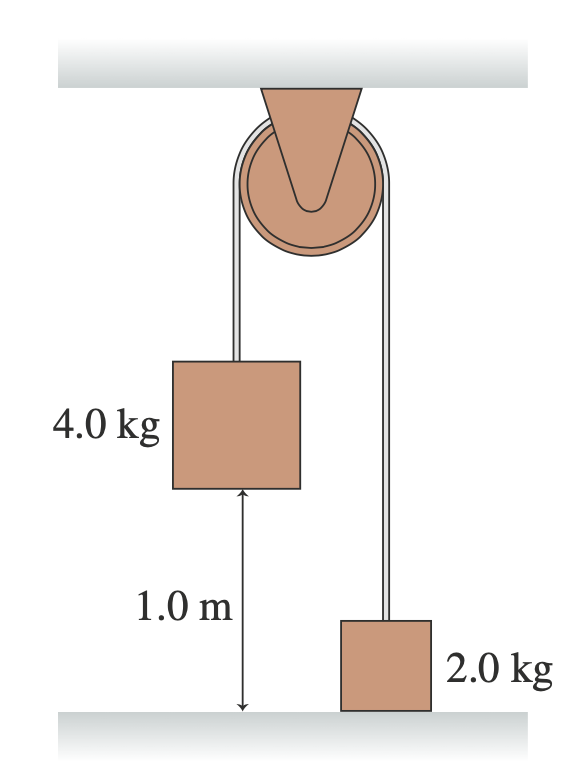
\includegraphics[scale = 0.45]{images/atwoopalaca.png}
\end{figure}


\subsection*{Hverfiþungi og hverfiþungavarðveisla}

\item \textit{(RK 12.46.)} Vínýlplata snýst með föstum hornhraða $33 \frac{1}{3}$ snúninga á mínútu. Massi vínýlplötu er $\SI{180}{g}$ og geisli hennar er $r = \SI{15.3}{cm}$.
\begin{enumerate}[label = \textbf{(\alph*)}]
    \item Hver er hornhraði vínýlplötunnar?
    \item Hver er hverfitregða vínýlplötunnar?
    \item Hver er hverfiþungi vínýlplötunnar?
    \item Nú er leirklessu með massa $m = \SI{240}{g}$ sleppt lóðrétt ofan á vínílplötuna í fjarlægð $d = \SI{7.5}{cm}$ frá miðju plötunnar. Hver verður sameiginlegur hornhraði kerfisins við það?
\end{enumerate}

\begin{minipage}{\linewidth}

\begin{wrapfigure}{r}{1.5in}
\vspace{-1.25cm}
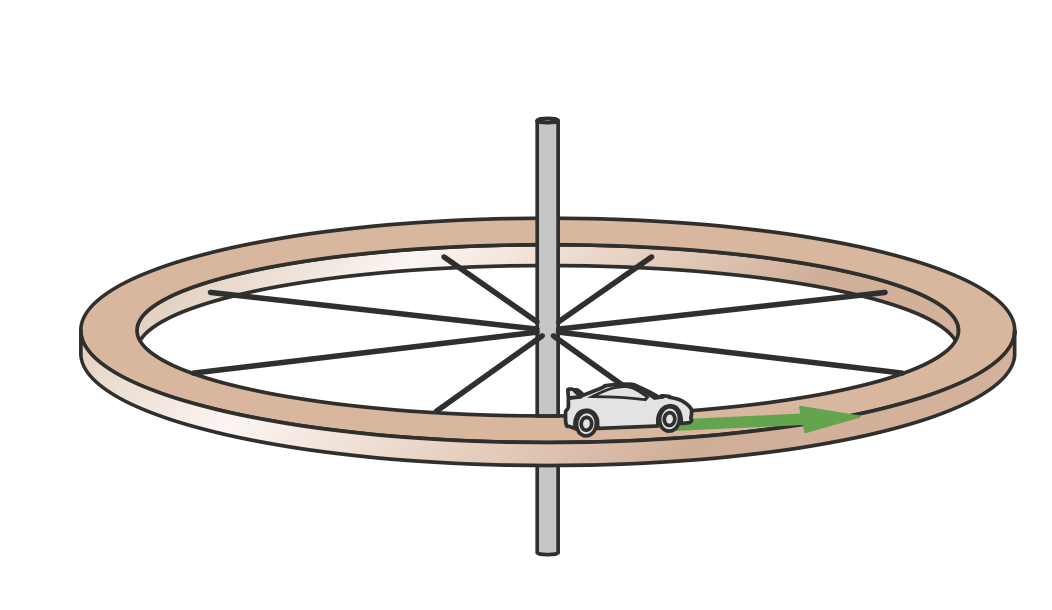
\includegraphics[width=2.2in]{images/bilahverfi.png}
\end{wrapfigure}

\item \textit{(RK 12.88.)} Lítll rafmagnsbíll með massa $m = \SI{200}{g}$ keyrir af stað úr kyrrstöðu á brautinni sem sést á myndinni hér til hægri. Geisli brautarinnar er $r = \SI{30}{cm}$ og massi hennar er $M = \SI{1.0}{kg}$. Litlar dældir eru í brautinni fyrir dekk bílsins þannig að hann keyri ekki útaf brautinni. Hver verður hornhraði brautarinnar eftir að bíllinn nær hámarkshraða, $v = \SI{0.75}{m/s}$, afstætt miðað við brautina.

\end{minipage}

\vspace{0.5cm}

\begin{minipage}{\linewidth}
\begin{wrapfigure}{r}{1.5in}
\vspace{-1.25cm}
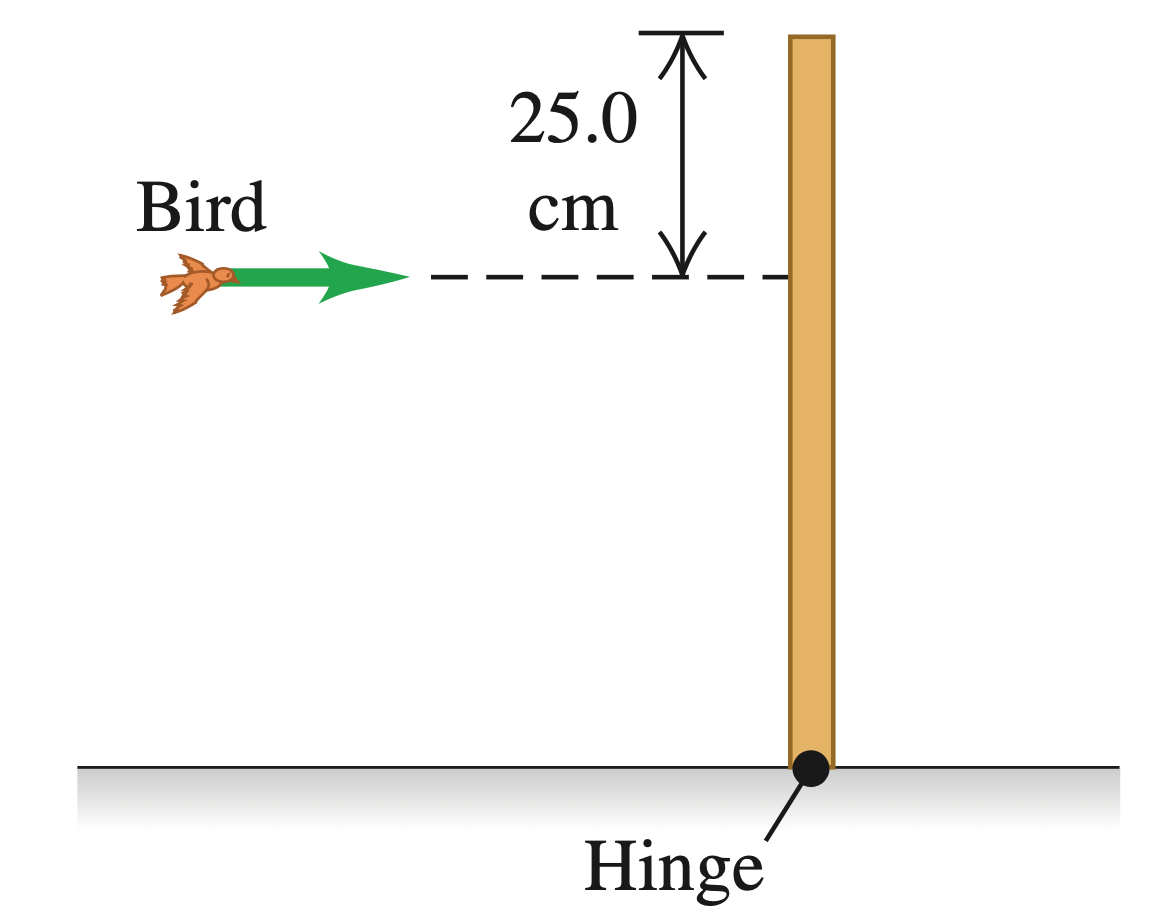
\includegraphics[width=2.2in]{images/fugl.png}
\end{wrapfigure}

\item Fugl með massa $m = \SI{500}{g}$ flýgur með láréttum hraða $v_0 = \SI{2.0}{m/s}$ og klessir á lóðrétta stöng í fjarlægð $y = \SI{25}{cm}$ frá toppi einsleitarar stangar sem hefur heildarlengd $\ell = \SI{0.75}{m}$ og massa $M = \SI{1.50}{kg}$. Stöngin er fest með hjörum um neðsta punktinn og getur aðeins snúist um þann ás. Áreksturinn er því miður þannig að aumingja fuglinn rotast og fellur meðvitundarlaus beint niður (með lárétta hraðann $v = 0$) eftir áreksturinn. Hver verður hornhraði stangarinnar rétt eftir áreksturinn? 

\end{minipage}

\vspace{0.5cm}

\item Tunglið er að fjarlægjast jörðina um $\SI{4}{cm}$ á ári. Þetta veldur því að jörðin fer að snúast hægar. Að lokum mun þetta leiða til þess að umferðartími tunglsins um jörðina verður sá sami og umferðartími jarðarinnar (samanber Karon, tungl Plútós). Í þessu dæmi munum við reyna að meta það hver lokasnúningshraði jarðarinnar verður. Látum $M_J$ tákna massa jarðarinnar, $M_T$ tákna massa tunglsins

\begin{enumerate}[label = \textbf{(\alph*)}]
    \item Finnið hornhraða jarðarinnar, $\omega_J$, og hornhraða tunglsins, $\omega_T$, um snúningsás jarðarinnar (núverandi).
    
    \item Finnið hverfitregðu jarðar, $I_J$, og núverandi hverfitregðu tungls, $I_{T1}$, um snúningsás jarðarinnar.
    
    \item Táknum nú lokahornhraða jarðarinnar með $\omega$ og lokafjarlægðina milli tungls og jarðar með $d$. \\ Notið þyngdarlögmál Newtons (ásamt því að tunglið sé á hringhreyfingu um jörðina) til að sýna:
    \begin{align*}
        \omega^2 d^3= GM_J
    \end{align*}
    
    \item Hverfiþungi kerfisins um snúningsás jarðarinnar er þá gefinn með $L_2 = I_{T2} \omega$ þar sem að $I_{T2}$ táknar hverfitregðu tunglsins eftir færslu tunglsins. Hér höfum við gert ráð fyrir því að $I_J \ll I_{T2}$ og að því megi hunsa liðinn $I_J\omega$. Nýtið ykkur varðveislu hverfiþungans ásamt niðurstöðunni í lið \textbf{(c)} til að finna bæði lokahornhraðan $\omega$ og lokafjarlægðina $d$.
    
    \item Hversu langur yrði sólarhringurinn þá?
\end{enumerate}

\begin{minipage}{\linewidth}
\begin{wrapfigure}{r}{1.5in}
\vspace{-0.75cm}
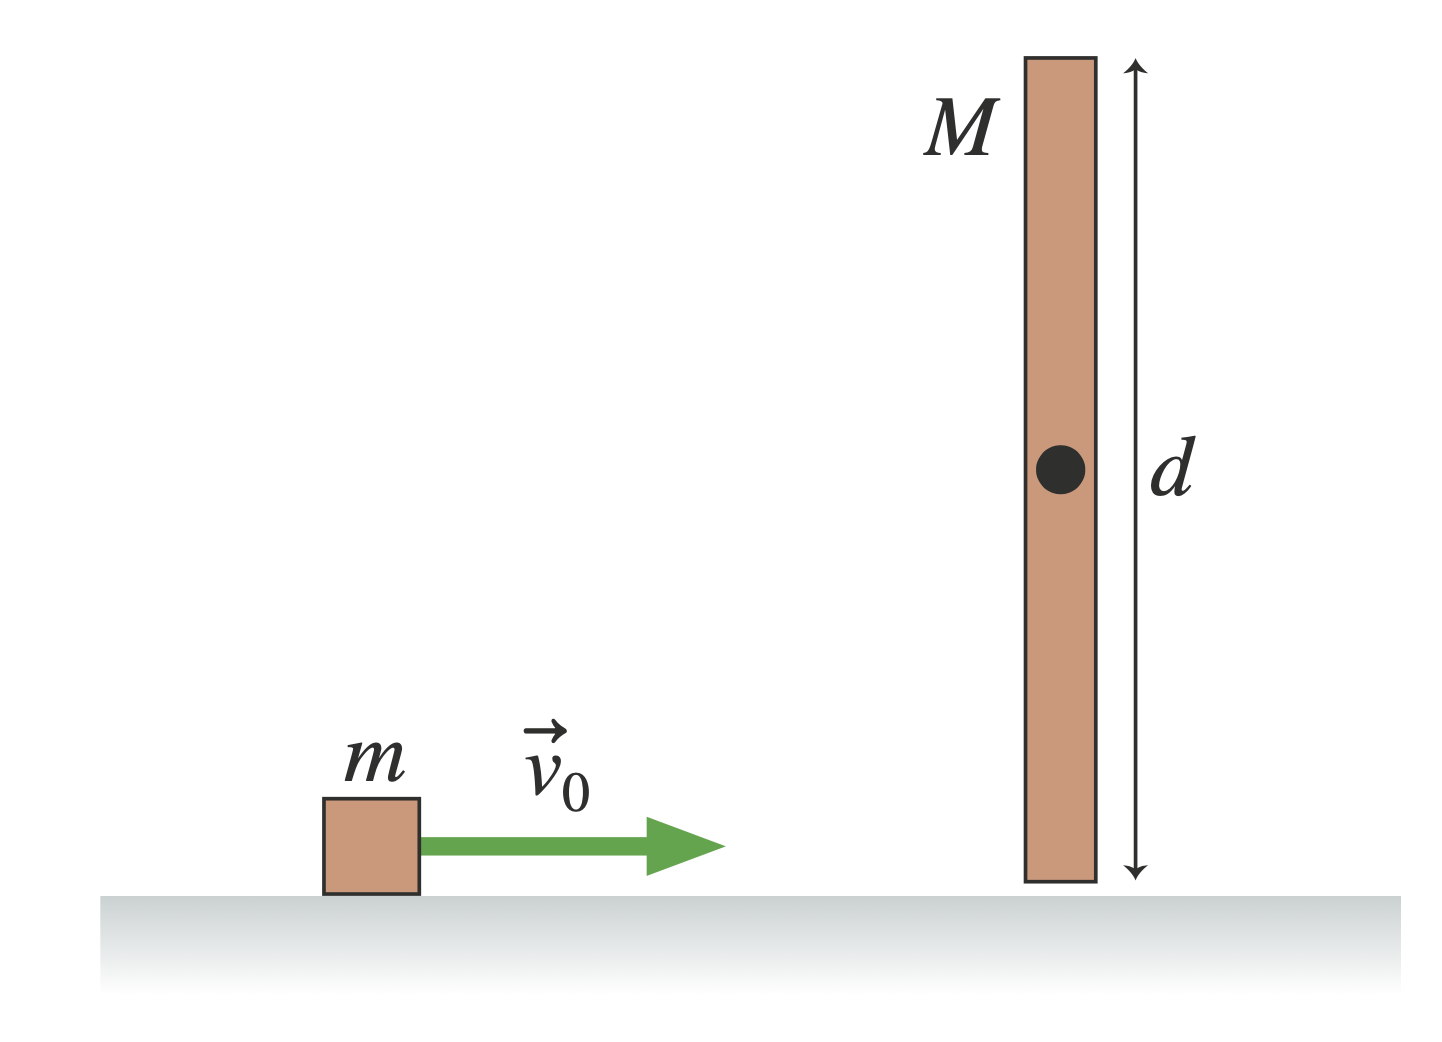
\includegraphics[width=2.2in]{images/klessahverfi.png}
\end{wrapfigure}

\item \textit{(RK 12.78.)} Byssukúlu með massa $m = \SI{10}{g}$ og upphafshraða $v_0 = \SI{400}{m/s}$ er skotið inn í hurð með massa $M = \SI{10}{kg}$ í láréttri fjarlægð $x = \SI{80}{cm}$ frá hjörum dyranna. Hurðin hefur breidd $b = \SI{95}{cm}$, þykkt $þ = \SI{5.0}{cm}$ og hæð $h = \SI{2.10}{m}$. Byssukúlan festist í hurðinni við áreksturinn. Hver verður hornhraði hurðarinnar eftir áreksturinn?

\item \textit{(RK 12.89.)} Kubbur með massa $m$ rennur eftir núninglausu yfirborði með upphafshraða $v_0$ þar til að hann lendir í fullkomlega fjaðrandi árekstri við neðsta hlutann á einsleitri stöng af lengd $d$ og með massa $M$. Nagli hefur verið settur í miðja stöngina þannig að hún getur aðeins snúist um miðju sína. Hver verður hraði kubbsins eftir áreksturinn?


\end{minipage}


\section*{Snúningsorka og snúningsvinnulögmálið}

\item \textit{(RK 12.69.)} Gegnheill sívalingur með massa $m$, geisla $r$ og af lengd $\ell$, rúllar án þess að renna meðfram láréttum fleti með hraða $\SI{5.0}{m/s}$ þar til að hann kemur að skábretti sem hallar um $\theta = \ang{22}$ miðað við lárétt. Hversu langt upp skábrettið kemst sívalingurinn áður en að hann byrjar að rúlla aftur niður?

\vspace{0.5cm}

\begin{minipage}{\linewidth}

\begin{wrapfigure}{r}{1.4in}
\vspace{-1cm}
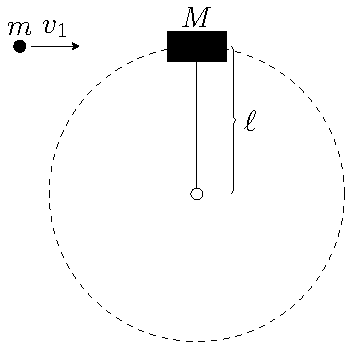
\includegraphics[width=2in]{images/angular_test.pdf}
\end{wrapfigure}

\item \textit{(Vorpróf 2018)} Byssukúlu með massa $m = \SI{4.8}{g}$ og hraða $v_1 = \SI{400}{m/s}$ er skotið inn í kubb með massa $M = \SI{2.2}{kg}$ sem hvílir á láréttum fleti. Núningsstuðullinn milli kubbsins og flatarins er $\mu = \SI{0.10}{}$. Kubburinn er festur við massalausa stöng og af lengd $\ell = \SI{50}{cm}$. Kerfið snýst um enda stangarinnar eftir hringferli eins og sýnt er á mynd.

\vspace{0.2cm}

\begin{enumerate}[label = \textbf{(\alph*)}]
    \item Finnið hornhraða kerfisins, $\omega_0$, rétt eftir að byssukúlan hefur stöðvast inni í kubbnum, t.d. með því að nota hverfiþungavarðveislu.
    \item Hversu langt ferðast kubburinn áður en núningur stöðvar hann? Svarið í radíönum og gráðum. Merkið inn á myndina staðsetningu þar sem kubburinn stöðvast.
\end{enumerate}
\end{minipage}

\vspace{0.5cm}

\begin{minipage}{\linewidth}

\begin{wrapfigure}{r}{1.5in}
\vspace{-1.25cm}
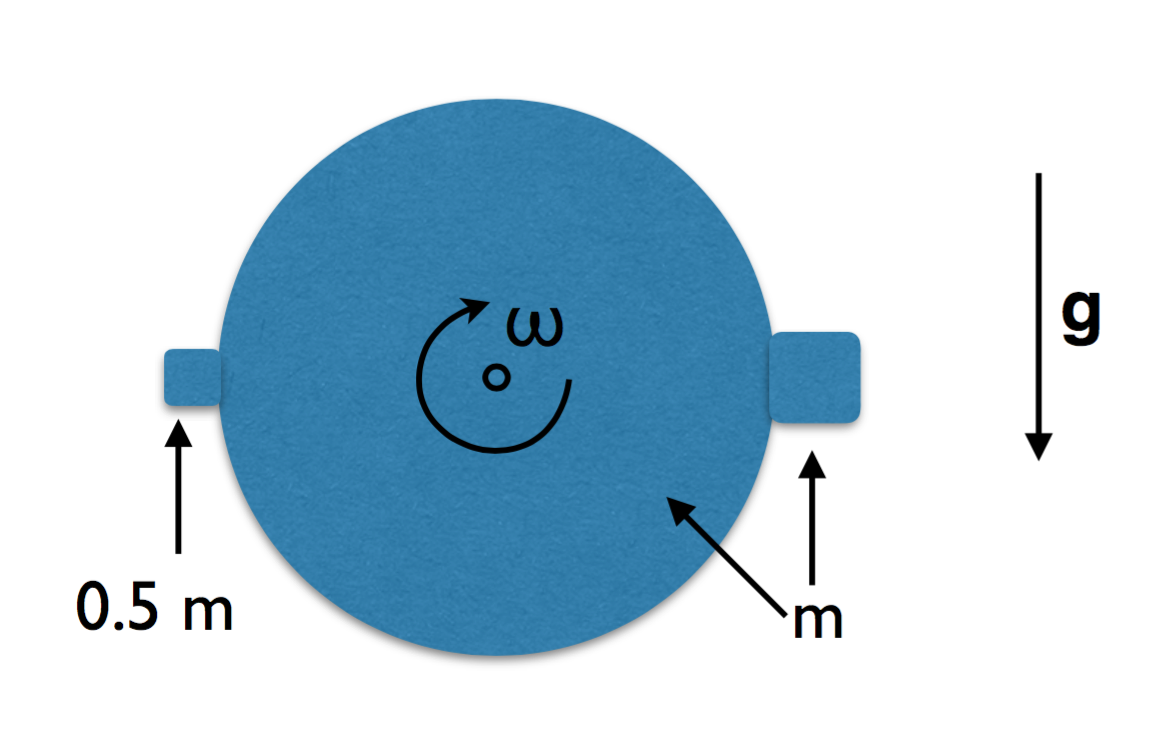
\includegraphics[scale = 0.25]{images/snuens.png}
\end{wrapfigure}

\item \textit{(Vorpróf 2018)} Diskur með massa $m = \SI{1.2}{kg}$ og geisla $r = \SI{50}{cm}$ getur snúist um núningslausann, láréttan ás (sem stefnir út úr blaðinu). Á diskinn eru festir tveir kubbar eins og sjá má á mynd. Vinstra meginn er festur kubbur með massann $\frac{1}{2}m = \SI{0.60}{kg}$ en hægra meginn er festur kubbur með massann $m = \SI{1.2}{kg}$.
\end{minipage}

\begin{enumerate}[label = \textbf{(\alph*)}]
    \item Finnið hornhröðun kerfisins rétt eftir að því er sleppt úr kyrrstöðu.
    \item Notið orkuvarðveislu til þess að finna hornhraða kerfisins þegar þyngri massinn er í lægstu stöðu og sá léttari er í efstu stöðu.
\end{enumerate}

\begin{minipage}{\linewidth}

\begin{wrapfigure}{r}{1.5in}
\vspace{-0.5cm}
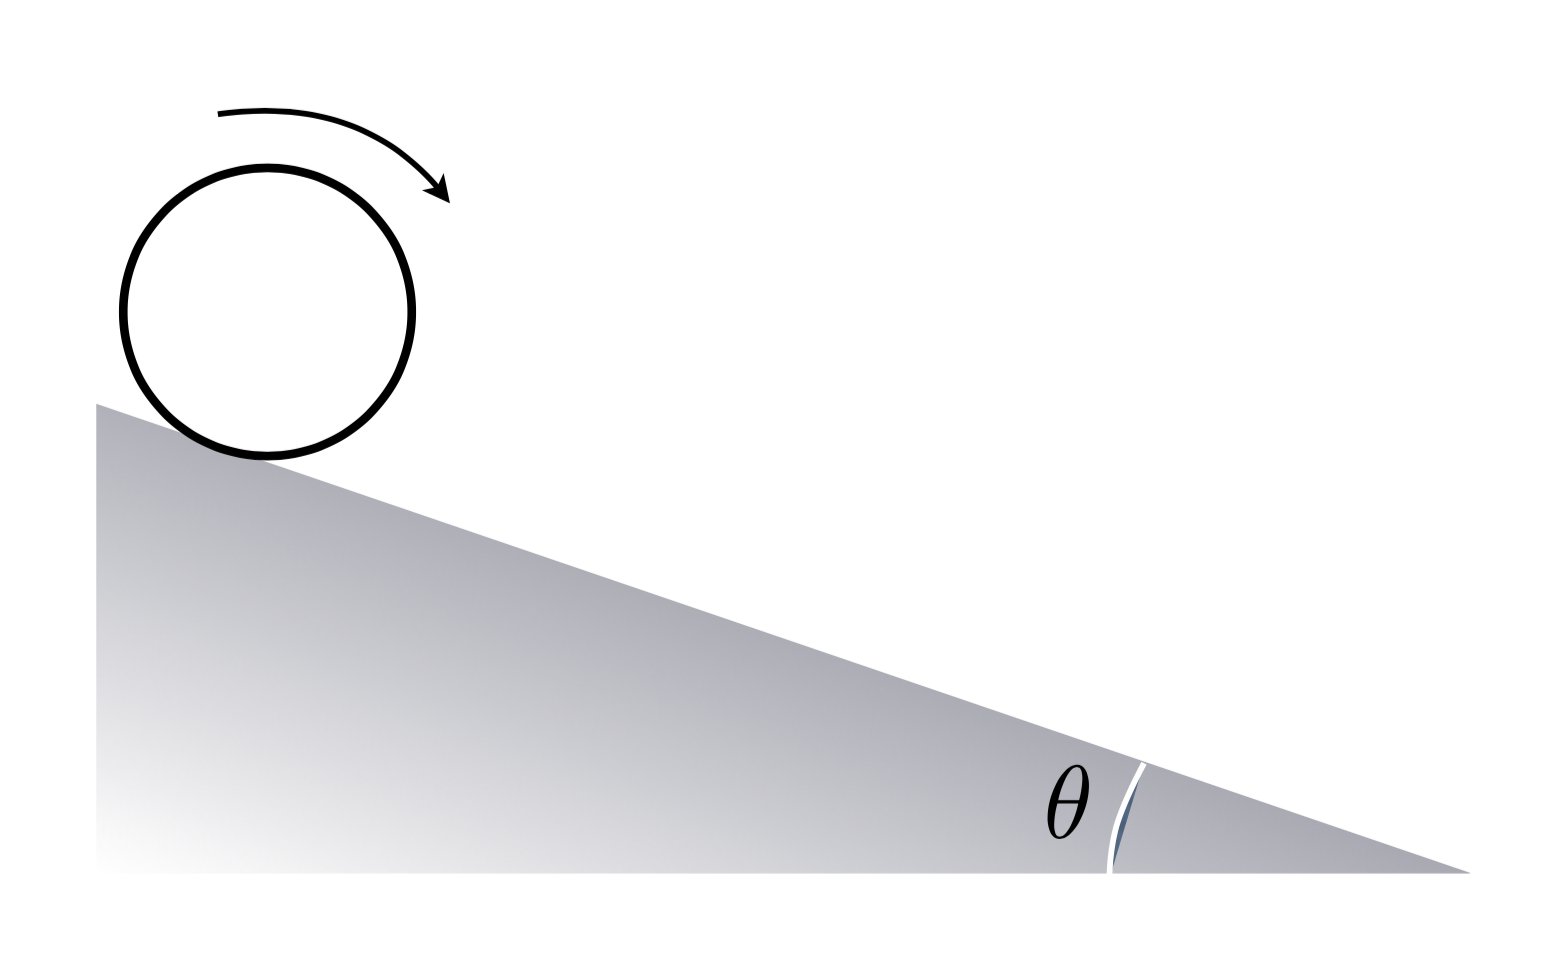
\includegraphics[width=2in]{images/rulla.png}
\end{wrapfigure}


\item Giftingarhringur með massa $\SI{6,0}{g}$ og geisla $\SI{7,0}{mm}$ rúllar án þess að renna úr kyrrstöðu niður skáplan sem hallar um $\theta = \SI{23}{\degree}$.
\end{minipage}

\begin{enumerate}[label = \textbf{(\alph*)}]
    \item Hver er hraði massamiðjunnar eftir að hringurinn hefur rúllað $\SI{2.0}{m}$ \\ niður eftir skáplaninu?
    
    \item Hver er lágmarksnúningsstuðull $\mu$ milli plans og gjarðar \\ til þess að gjörðin rúlli án þess að renna?
\end{enumerate}

\item \textit{(RK 12.74.)} Blýantur með massa $m$ og lengd $\ell$ stendur lóðréttur á láréttu borði. Einhver ýtir örlítið við blýantinum þannig að hann byrjar að detta. Hver verður hornhraði blýantsins rétt áður en að hann lendir á jörðinni? Gerum ráð fyrir að neðsti hluti blýantsins haldist í snertingu við borðið þar til að hann lendir.

\vspace{0.5cm}


\begin{minipage}{\linewidth}

\begin{wrapfigure}{r}{1.5in}
\vspace{-0.75cm}
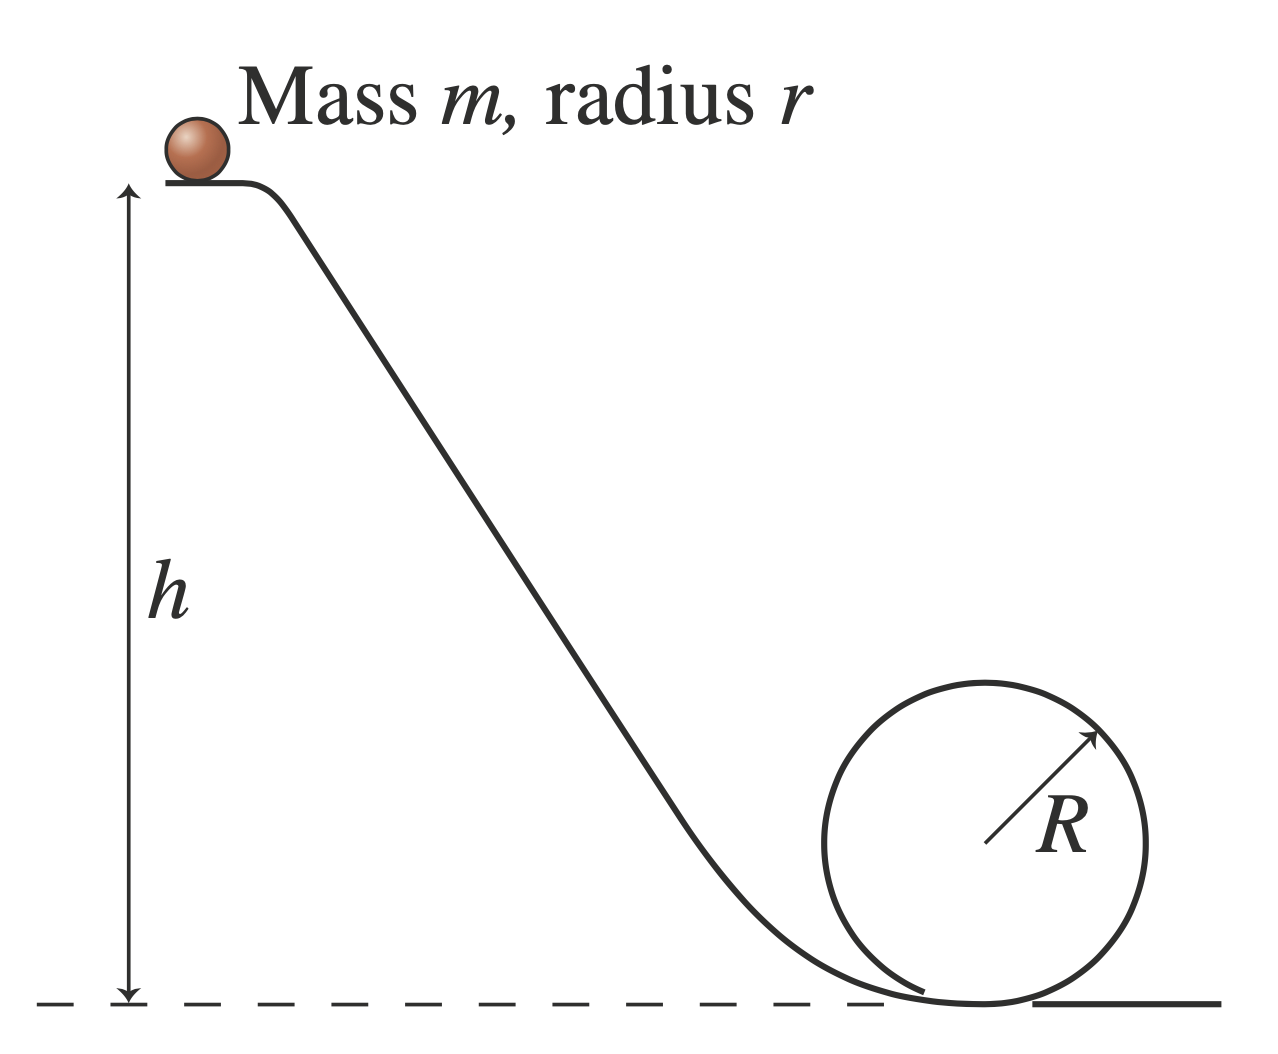
\includegraphics[width=1.5in]{images/usapho.png}
\end{wrapfigure}


\item \textit{(RK 12.75.)} Glerkúla með massa $m$ og geisla $r$ rúllar án þess að renna niður brautina sem sést á myndinni hér til hægri. Hvert er minnsta gildið á hæðinni, $h$, þannig að kúlan komist allan hringinn (með geisla $R$) án þess að detta í efstu stöðu?
\end{minipage}



\newpage


\subsection*{Erfið dæmi}


\item Í borgarumsátrum miðalda voru valslöngvur ómissandi tæki, en þær valslöngvur sem við þekkjum best eiga líklegast rætur sínar að rekja til soldánadæmis Ayyubída á 12. öld e.o.t. (en voru mögulegu fundnar upp fyrst í Austur Rómarveldi á 11. öldinni) og breiddust þaðan út til Evrópu og Kína.
Athugum eiginleika einfaldaðrar valslöngvu, sjá myndir~\ref{rest} og~\ref{throw}.
Valslöngvan virkar þannig að massalaus \textit{armur} af lengd \(L\) er festur á \textit{öxul} í hæð \(h\) frá jörðinni sem skiptir arminum í \textit{kastarm} af lengd \(\ell_1\) og \textit{fallarm} af lengd \(\ell_2\).
Við enda kastarmsins er fest massalaus \textit{karfa} sem geymir stein af massa \(m\).
Við fallarminn er fest \textit{mótvigt} af massa \(M\).
Gerum ráð fyrir að armurinn bogni ekki, að enginn núningur sé í kerfinu og hunsum massa allra festinga og aukahluta sem gætu komið við sögu.

\begin{figure}[ht]
\begin{minipage}[b]{0.45\linewidth}
    \centering
    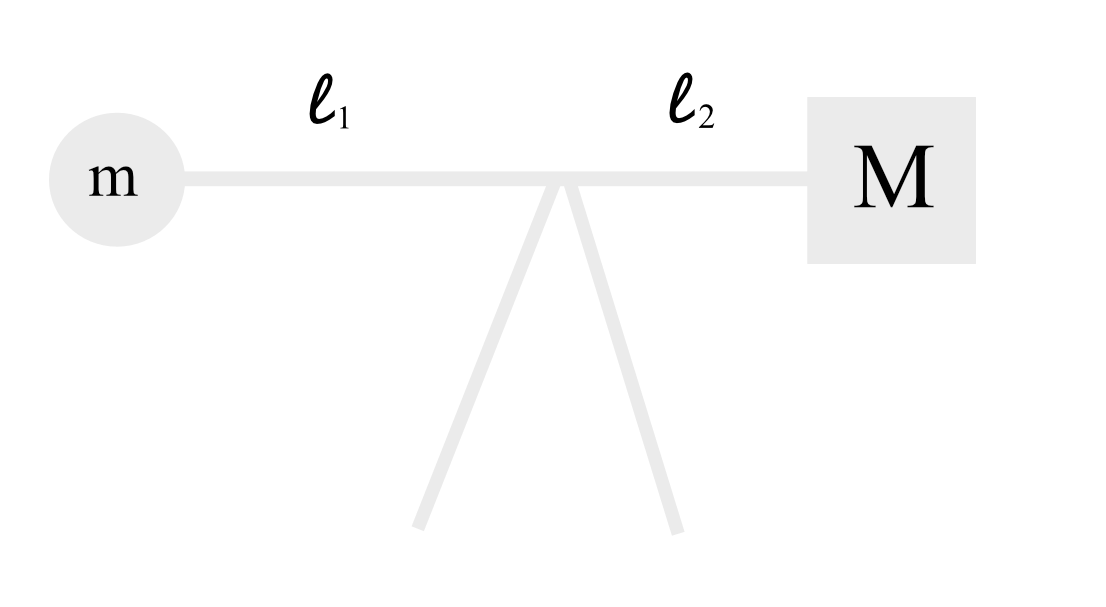
\includegraphics[scale=0.65]{images/massistong.png}
    \caption{Valslöngva fest í hvíldarstöðu.}
    \label{rest}
\end{minipage}
\hspace{0.5cm}
\begin{minipage}[b]{0.65\linewidth}
    \centering
    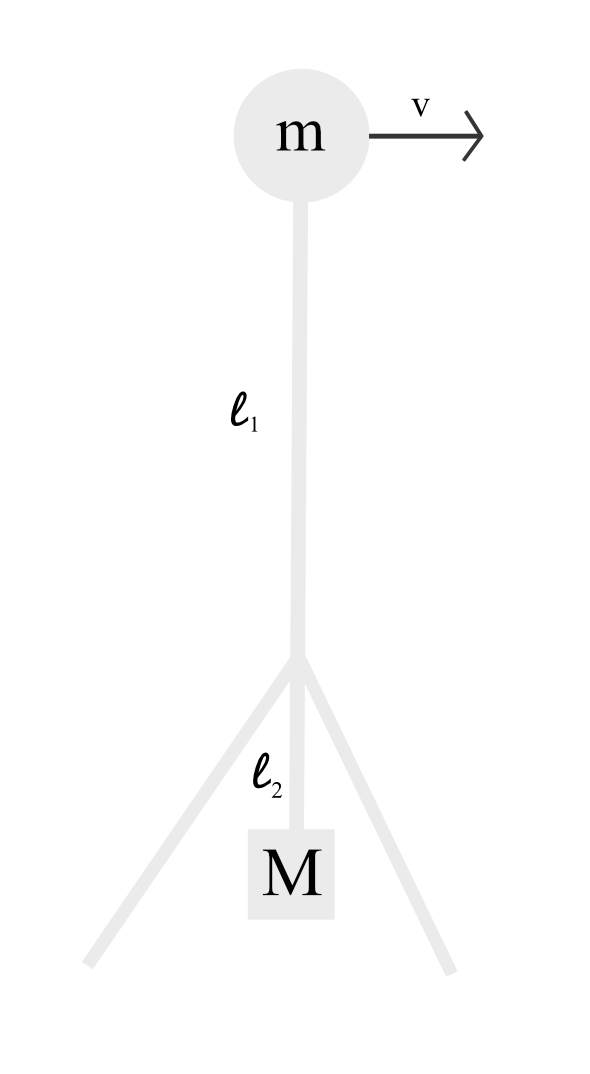
\includegraphics[scale = 0.8]{images/al.png}
    \caption{Valslöngva þegar steinninn sleppur.}
    \label{throw}
\end{minipage}
\end{figure}

\begin{enumerate}[label=\textbf{(\alph*)}]
    \item Finnið hverfitregðu kerfisins, $I$, um snúningsásinn, sem fall af $m, M, \ell_1, \ell_2$ og þekktum föstum.
    %Lausn: m\ell_1^2 + M\ell_2^2
    
    \item Steininum er sleppt þegar heildarvægið á arminn er núll. Finnið hornhraða steinsins, \(\omega\), þegar hann sleppur úr körfunni sem fall af $m, M, \ell_1, \ell_2, I$ og þekktum föstum með því að nota orkuvarðveislu.
    % Lausn: \ell_1\sqrt{\frac{2g}{I}(M\ell_2 - m\ell_1}

    
    \item Finnið hversu langt steinninn fer áður en hann lendir á jörðinni sem fall af $m, M, \ell_1, \ell_2, h, I$ og þekktum föstum.
    % Lausn: 2\ell_1\sqrt{\frac{(M\ell_2 - m\ell_1)(\ell_1 + h}{m\ell_1^2 + M\ell_2^2}}
    
    \item Látum massa steinsins vera \SI{45}{kg}, massa mótvigtarinnar vera \SI{2000}{kg}, lengd kastarmsins vera \SI{12}{m}, lengd fallarmsins vera \SI{2.0}{m} og hæð öxulsins vera \SI{6.0}{m}. Hversu langt kastast steinninn?
    % Lausn: 50 m
\end{enumerate}

\item Skoðum kústskaft með einsleita massadreifingu sem hefur lengd $L$ og massa $M$. Gerum ráð fyrir að þykkt þess sé óveruleg og það standi lóðrétt í jafnvægi á sléttum fleti. Enginn núningur verkar milli flatar og kústskafts. Hleypt er af byssu nálægt skaftinu og henni haldið þannig að þegar byssukúlan festist í skaftinu er kúlan í hæð $x$ yfir miðju skaftsins og hraði kúlunnar $v$ er í lárétta stefnu. Massi byssukúlunnar er $m$. 

\begin{enumerate}[label = \textbf{(\alph*)}]
    \item Notið skriðþungavarðveislu til að finna línulegan hraða skaftsins, $u$, eftir áreksturinn.
    
    \item Látum $y_1$ tákna massamiðju skaftsins fyrir áreksturinn og látum $y_2$ tákna massamiðju skaftsins eftir áreksturinn. Ákvarðið bæði $y_1$ og $y_2$ ásamt stærðinni $y := y_2-y_1$.
    
    \item Finnið hverfiþungann, $L_{1}$, fyrir áreksturinn um ás sem liggur í gegnum nýju massamiðjuna.
    
    \item Finnið hverfitregðu stangarinnar, $I_y$, um ás í gegnum nýju massamiðjuna, sem fall af $m, M, x, L$.
    
    \item Nýtið ykkur hverfiþungavarðveislu til þess að finna hornhraða stangarinnar, $\omega$, um massamiðjuna.
    
    \item Finnið $x$ sem fall af $L, M, m$ og $v$ þ.a. neðsti punktur skaftsins verði kyrr rétt eftir áreksturinn.
\end{enumerate}

\end{enumerate}


\section*{Svör}

\begin{enumerate*}[label = \vspace{0.15cm} \textbf{(\arabic*)}]
  \item $\alpha = \SI{410}{rad/s^2}$, $\frac{\Delta \theta}{2\pi} = \SI{18.3}{\text{snúningar}}$.
  \item $\alpha = \SI{-0.43}{rad/s^2}$, $\omega = \SI{18.3}{rad/s}$, $\frac{\Delta \theta}{2\pi} = \SI{125}{\text{snúningar}}$.
  \item $\omega_{\text{innri}} = \SI{50}{rad/s}$, $\omega_{\text{ytri}} = \SI{22}{rad/s}$, $s = \SI{5.6}{km}$.
  \item $x_a - R = \frac{M_T}{M_J + M_T}d = \SI{4.67e6}{m}$, $x_b = \frac{M_J}{M_S + M_J}R = \SI{4.50e5}{m}$, $x_c = \frac{M_J R + M_T (R+d)}{M_S + M_J + M_T} = \SI{4.56e5}{m}$.
  \item $\smqty(x_{\text{cm}} \\ y_{\text{cm}}) = \smqty(\SI{1.7}{cm} \\ \SI{3.3}{cm})$. \item $I_a = \frac{2}{5}mR^2$, $I_b = mR^2$, $I_c = \frac{1}{12}mL^2$, $I_d = \frac{1}{9}mL^2$.
  \item $\smqty(x_{\text{cm}} \\ y_{\text{cm}}) = \smqty(\SI{6.0}{cm} \\ \SI{4.0}{cm})$, $I_A = \SI{2.0e-3}{kg.m^2}$, $I_{BC} = \SI{1.3}{kg.m^2}$.
  \item $I_{\text{hjarir}} = \SI{4.7}{kg.m^2}$, $I_{\text{lárétt}} = \SI{24.6}{kg.m^2}$.
  \item $I_{\text{miðja}} = \SI{1.23}{kg.m^2}$, $x_{\text{cm}} = \SI{-14}{cm}$, $I_{\text{cm}} = \SI{1.1}{kg.m^2}$.
  \item $I_J = \SI{8.0e37}{kg.m^2}$.
  \item $\tau_{\text{heild}} = \SI{-0.40}{Nm}$, $\alpha = \SI{330}{rad/s^2}$.
  \item $\tau_a = \SI{5.0}{Nm}$, $\tau_b = \SI{5.0}{Nm}$. \item $T = \SI{15000}{N}$. 
  \item $d_n \leq \frac{(n+1)}{4}\ell$.
  \item $T = \SI{642}{N}$, $F_x = \SI{526}{N}$, $F_y = \SI{1.98}{N}$.
  \item $a = \SI{4.73}{m/s^2}$, $\alpha = \SI{33.8}{rad/s^2}$.
  \item $T_A = \SI{95}{N}$, $T_B = \SI{121}{N}$, $\alpha = \SI{7.1}{rad/s^2}$.
  \item $T_1 = \SI{196}{N}$, $T_2 = \SI{344}{N}$, $\alpha = \SI{9.1}{rad/s^2}$.
  \item $m_s \leq \SI{30.5}{kg}$.
  \item $t = \SI{0.95}{s}$.
  \item $\omega_1 = \SI{3.49}{rad/s}$, $I_1 = \SI{2.11e-3}{kg.m^2}$, $L_1 = \SI{7.35e-3}{kg.m^2}$, $\omega_2 = \SI{2.12}{rad/s}$.
  \item $\omega_{\text{braut}} = \SI{0.42}{rad/s}$.
  \item $\omega_2 = \SI{1.78}{rad/s}$.
  \item $\omega_J = \SI{7.27e-5}{rad/s}$, $\omega_T = \SI{2.69e-6}{rad/s}$, $I_J = \SI{8.0e37}{kg.m^2} \approx \SI{9.7e37}{kg.m^2}$, $I_{T_{1}} = \SI{1.1e40}{kg.m^2} \gg I_J$, $L_1 = \SI{3.5e34}{kg.m^2}$, $d = \SI{5.7e8}{m} = \SI{1.5}{}R_T$, $\omega = \SI{1.5e-6}{rad/s}$, $T = \SI{49}{dagar}$.
  \item $\omega_2 = \SI{1.06}{rad/s}$.
  \item $v = \frac{m-\frac{1}{3}M}{m+\frac{1}{3}M}v_0$.
  \item $h = \SI{1.9}{m}$.
  \item $\omega_0 = \SI{1.74}{rad/s}$, $\Delta \theta = \SI{0.77}{rad} = \ang{44}$.
  \item $\alpha = \SI{4.91}{rad/s^2}$, $\omega = \SI{3.1}{rad/s}$.
  \item $v_{\text{cm}} = \SI{4.43}{m/s}$, $\mu \geq \frac{\sigma}{1+\sigma}\tan\theta = \SI{0.21}{}$.
  \item $\omega = \sqrt{\frac{3g}{\ell}}$. \item $h > \frac{27}{10}R$.
  \item $I = \SI{14500}{kg.m^2}$, $\omega = \SI{2.16}{rad/s}$, $x = \SI{49.5}{m}$.
  \item $u = \frac{mv}{m+M}$, $y = \frac{mx}{m+M}$, $L_1 = \frac{mM}{m+M}vx$, $I_y = \frac{1}{12}ML^2 + \frac{mM}{m+M}x^2$, $\omega = \frac{L_1}{I_y}$, $x = \frac{1}{6}L$.
\end{enumerate*}


\newpage